\chapter{Árvores Rubro-Negras}
\chaplabel{redblack}

\index{árvore de busca binária!rubro-negra}%
\index{árvore rubro-negra}%
Neste capítulo apresentamos as árvores rubro-negras, uma versão das árvores binárias de busca com altura logarítmica. As árvores rubro-negras são uma das estruturas de 
dados mais utilizadas. Elas aparecem como a principal estrutura de busca em 
muitas implementações de bibliotecas, incluindo a Java Collections Framework e
várias implementações da C++ Standard Template Library. Elas também são
utilizadas no kernel do sistema operacional Linux. Existem várias
razões para a popularidade das árvores rubro-negras:
\begin{enumerate}
	\item Uma árvore rubro-negra com #n# elementos tem altura de no máximo $2\log #n#$.
	\item As operações #add(x)# e #remove(x)# em uma árvore rubro-negra são executadas em
	temp $O(\log #n#)$ no \emph{pior caso}.
	\item O número de rotações amortizadas realizadas durante uma operação #add(x)#
	ou #remove(x)# é constante.
\end{enumerate}
As duas primeiras dessas propriedades já colocam as árvores rubro-negras
à frente de skiplists, treaps, e árvores scapegoat.
Skiplists e treaps dependem de randomização, e seus tempos de execução 
$O(\log #n#)$ são apenas esperados. As árvores scapegoat têm limite de altura
garantido, mas as operações #add(x)# e #remove(x)# executam apenas em tempo 
amortizado $O(\log#n#)$. A terceira propriedade é a cereja do bolo. 
Ela nos diz que o tempo necessário para adicionar ou remover um elemento #x# é
limitado pelo tempo necessário para encontrar #x#.\footnote{Note que, nesse sentido,
	as skiplists e treaps também têm essa propriedade. 
	Veja os exercicios ~\ref{exc:skiplist-changes} e \ref{exc:treap-rotates}.}

No entanto, as propriedades legais das árvores rubro-negras vêm com um preço:
complexidade de implementação. Manter um limite de $2\log #n#$ na altura não é fácil. 
Isso exige uma análise cuidadosa de vários casos.
Devemos garantir que a implementação faça exatamente a coisa certa
em cada caso. Uma mudança de cor ou rotação mal feita produz
um bug que pode ser muito difícil de entender e rastrear.

Em vez de pular diretamente para a implementação das árvores rubro-negras,
primeiro passaremos alguma base sobre uma estrutura de dados relacionada:
a árvore 2-4. Isso dará uma visão de como as árvores rubro-negras 
foram descobertas e porque a manutenção eficiente delas pode ser possível.

\section{Árvores 2-4}
\seclabel{twofour}

Uma árvore 2-4 é uma árvore enraizada com as seguintes propriedades:
\begin{prp}[Altura]
	Todas as folhas têm a mesma profundidade.
\end{prp}
\begin{prp}[grau]
	Cada nó interno tem 2, 3 ou 4 filhos.
\end{prp}
Um exemplo de uma árvore 2-4 é mostrado na \figref{twofour-example}.
\begin{figure}
	\begin{center}
		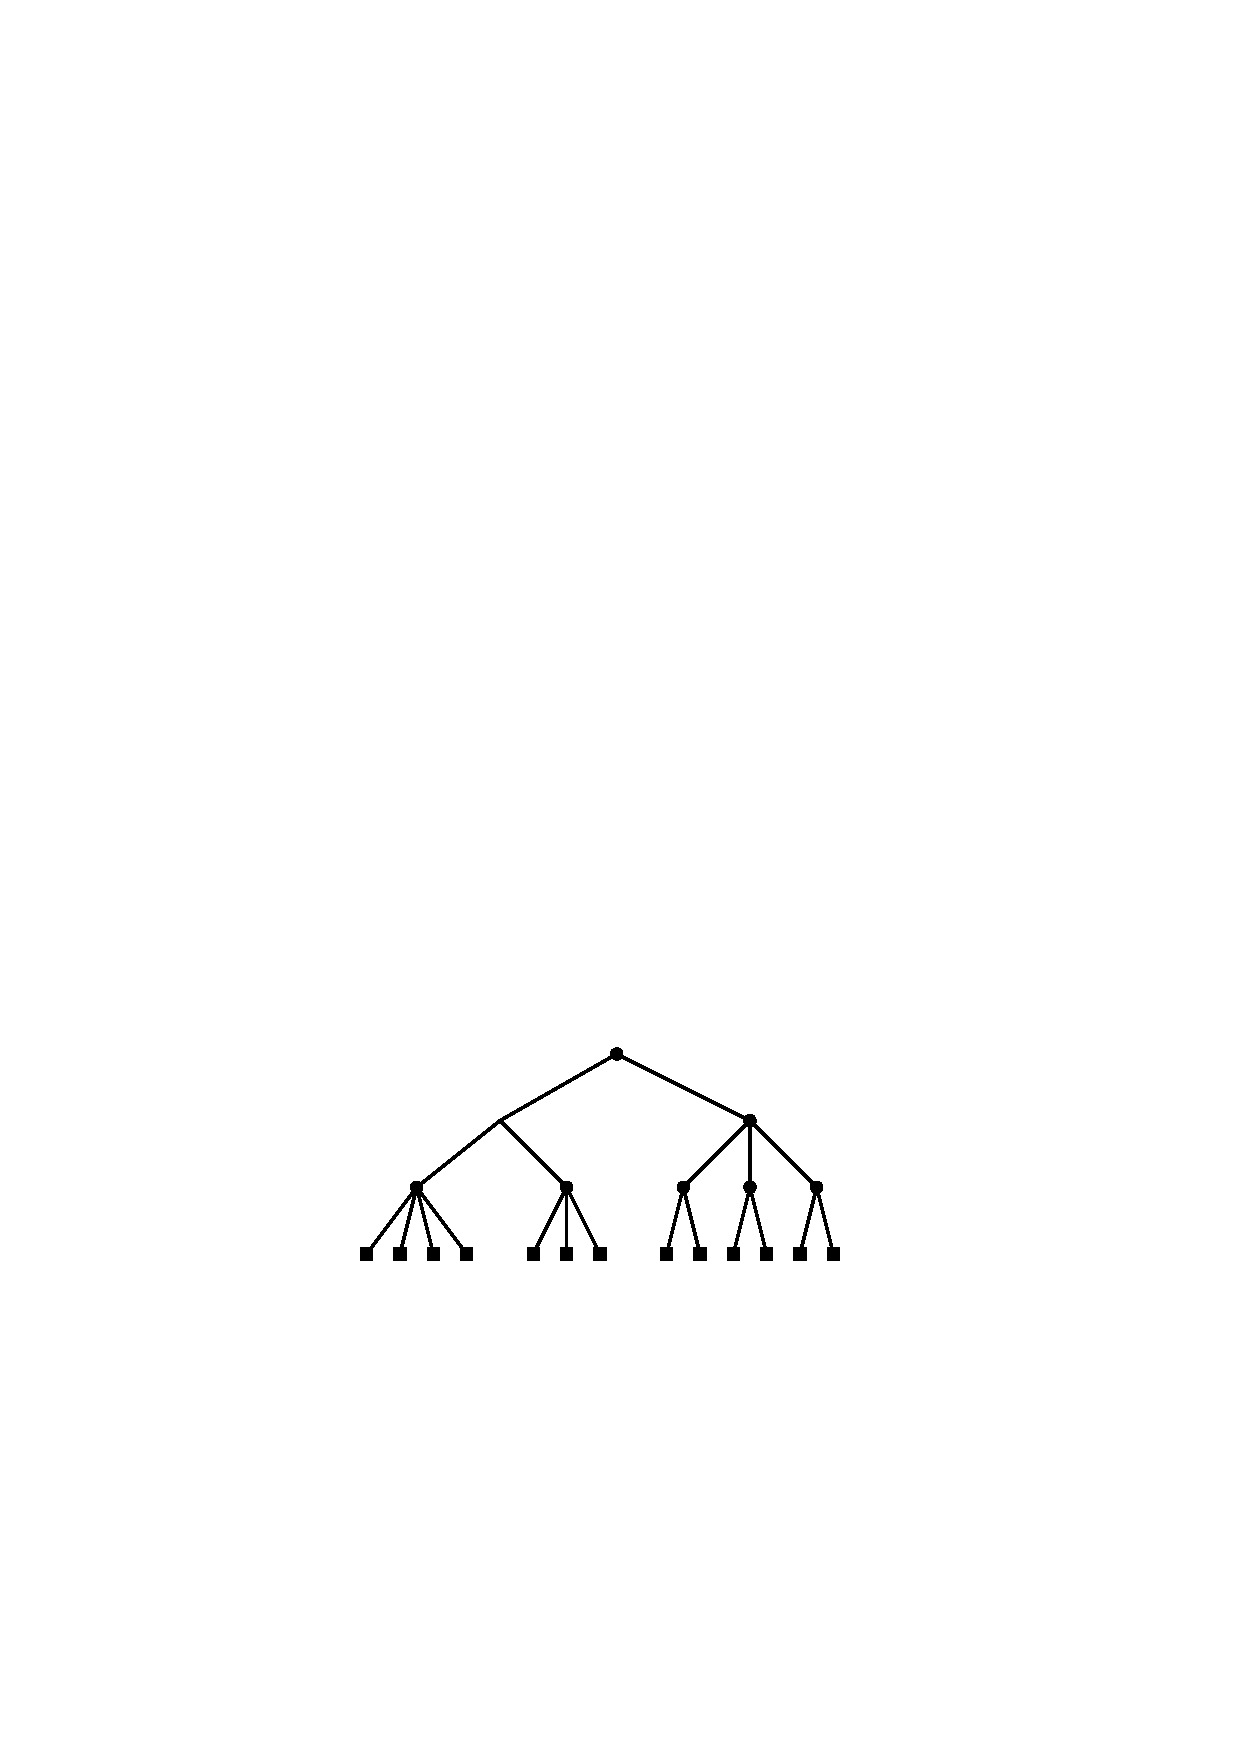
\includegraphics[scale=0.90909]{figs/24rb-2}
	\end{center}
	\caption{Uma árvore 2-4 de altura 3.}
	\figlabel{twofour-example}
\end{figure}
As propriedades das árvores 2-4 implicam que sua altura é logarítmica 
no número de folhas:
\begin{lem}\lemlabel{twofour-height}
	Uma árvore 2-4 com #n# folhas tem altura máxima de $\log #n#$.
\end{lem}

\begin{proof}
	O limite inferior de 2 no número de filhos de um nó interno
	implica que, se a altura de uma árvore 2-4 for $h$, então ela tem no mínimo
	$2^h$ folhas. Em outras palavras,
	\[
	#n# \ge 2^h \enspace .
	\]
	Tirando o log de ambos os lados desta desigualdade resulta em $h \le \log #n#$.
\end{proof}

\subsection{Adicionando uma folha}

Adicionar uma folha a uma árvore 2-4 é fácil (veja \figref{twofour-add}). Se nós
queremos adicionar uma folha #u# como filho de algum nó #w# no penúltimo
nível, então simplesmente fazemos #u# um filho de #w#. Isso certamente mantém
a propriedade da altura, mas poderia violar a propriedade do grau; se #w#
tinha quatro filhos antes de adicionar #u#, então #w# agora tem cinco filhos.
Neste caso, nós \emph{dividimos}
\index{split}%
#w# em dois nós, #w# and #w#', tendo
dois e três filhos, respectivamente.
Mas agora #w#' não tem pai,
então, recursivamente, fazemos #w#' um filho do pai de #w#. Novamente, isso pode
fazer com que o pai de #w# tenha muitos filhos, caso em que o dividimos.
Este processo continua até alcançar um nó com menos de quatro filhos,
ou até dividir a raiz, #r#, em dois nós #r# e #r'#. Nesse
último caso, criamos uma nova raiz que tem #r# e #r'# como filhos.
Isso aumenta a profundidade de todas as folhas simultaneamente e, portanto, mantém
a propriedade da altura.

\begin{figure}
	\begin{center}
		\begin{tabular}{c}
			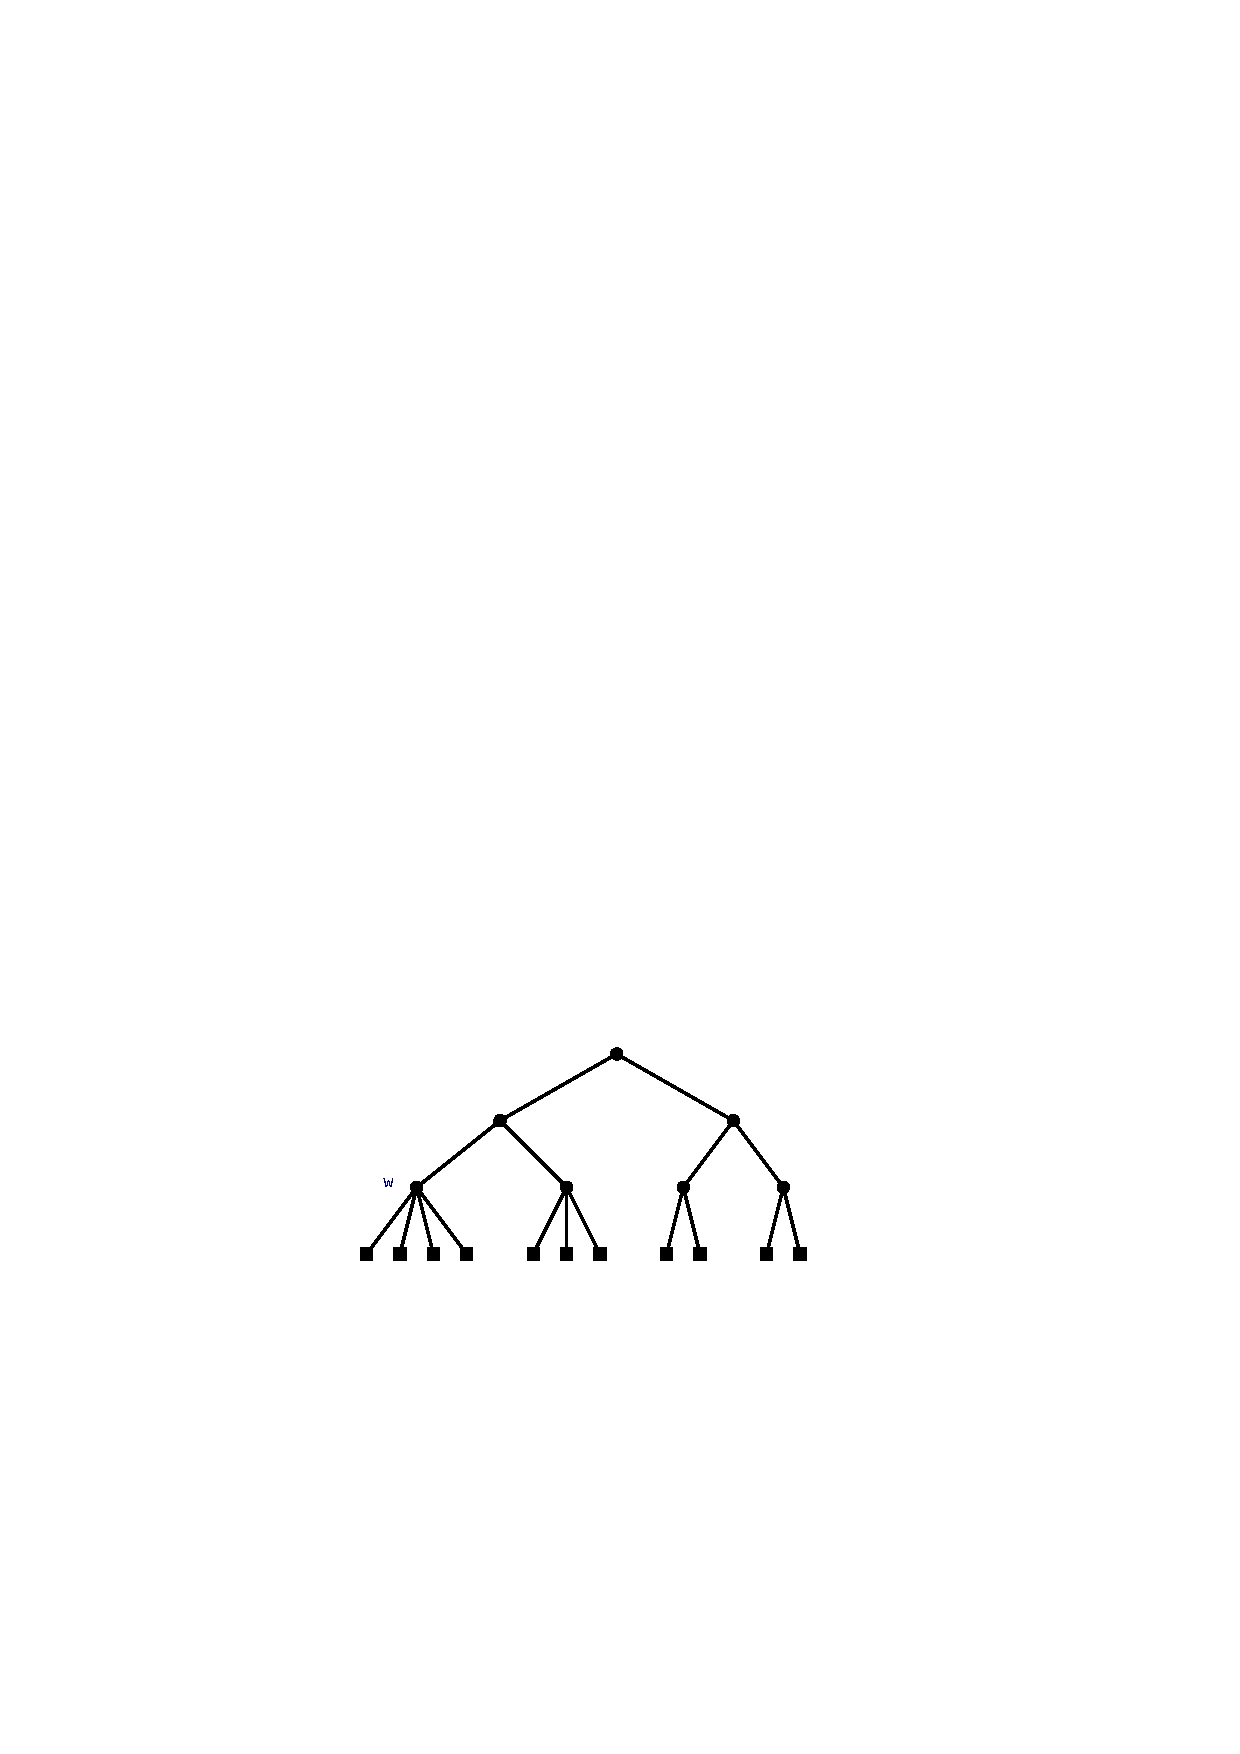
\includegraphics[scale=0.90909]{figs/24tree-add-1} \\
			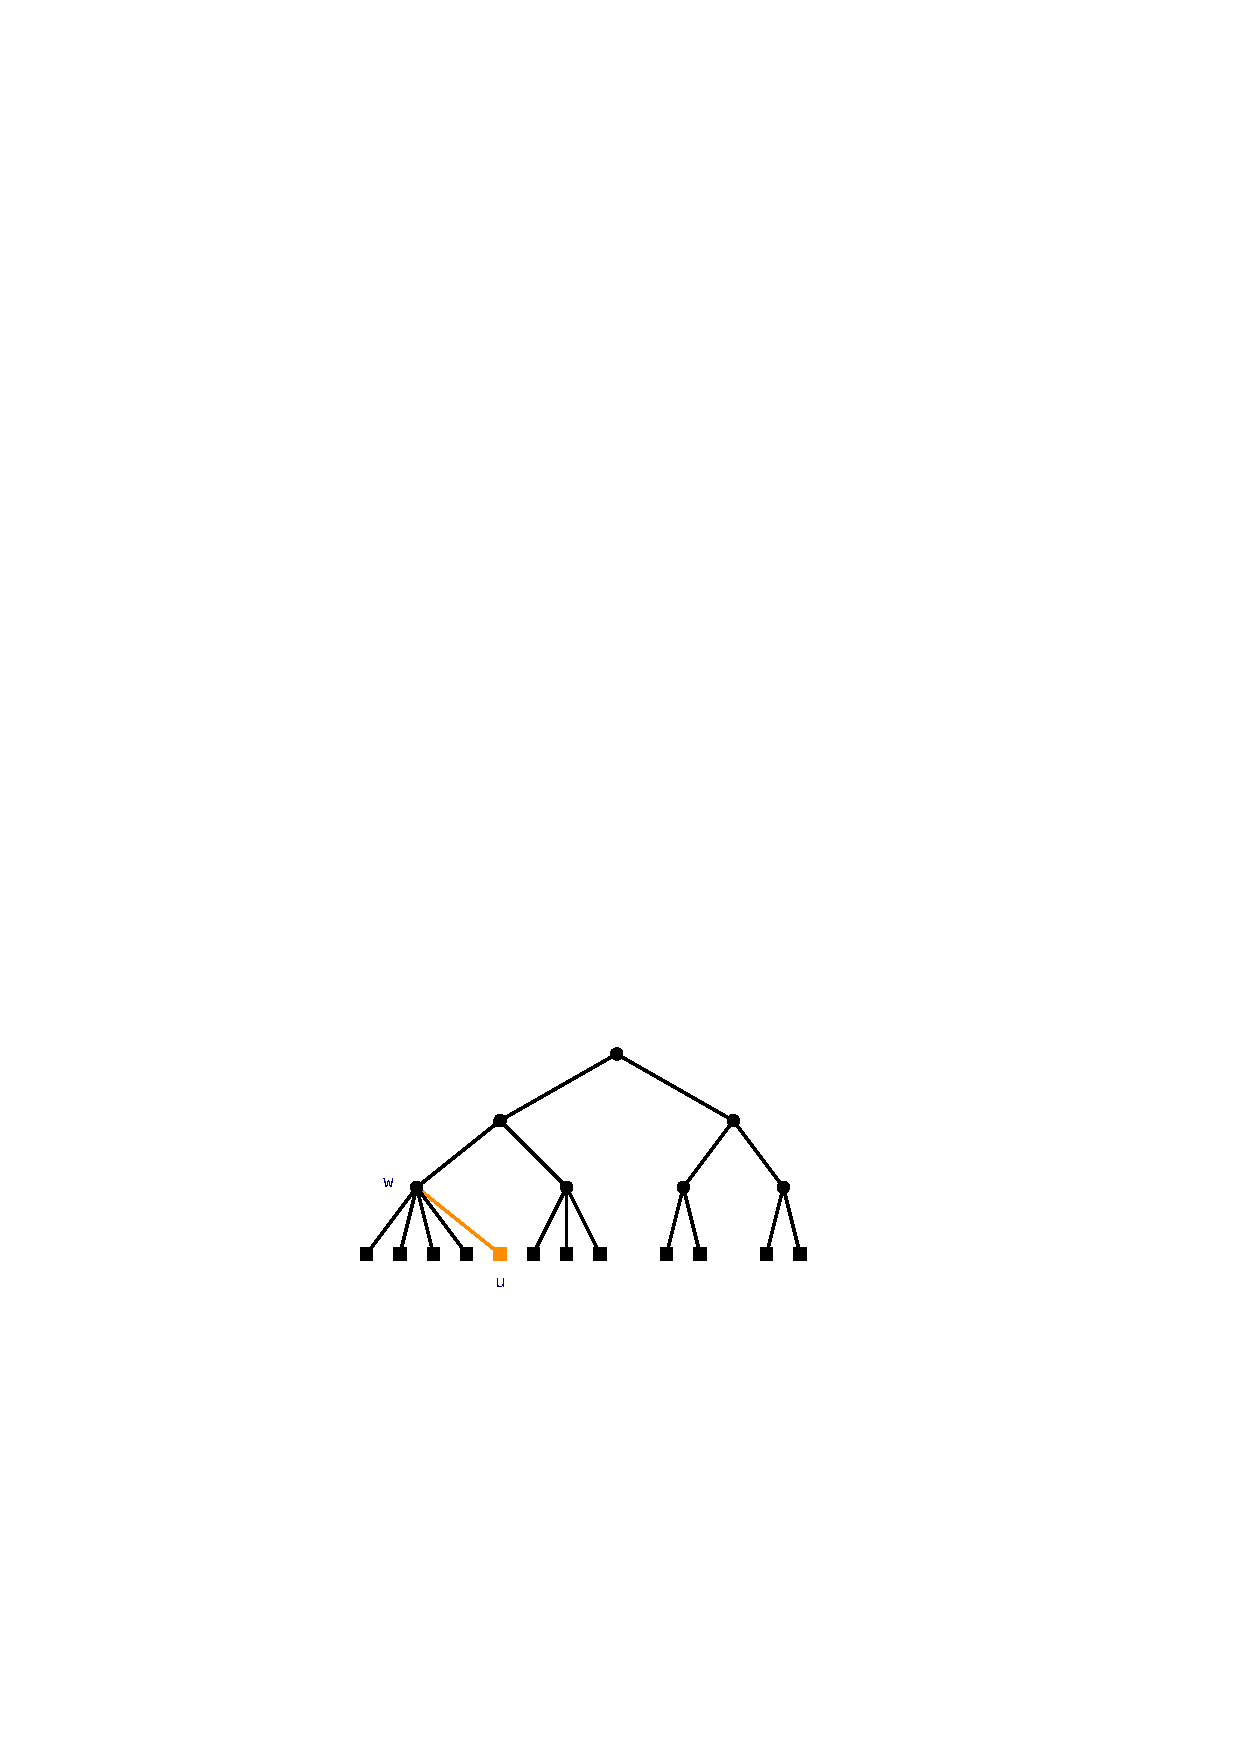
\includegraphics[scale=0.90909]{figs/24tree-add-2} \\
			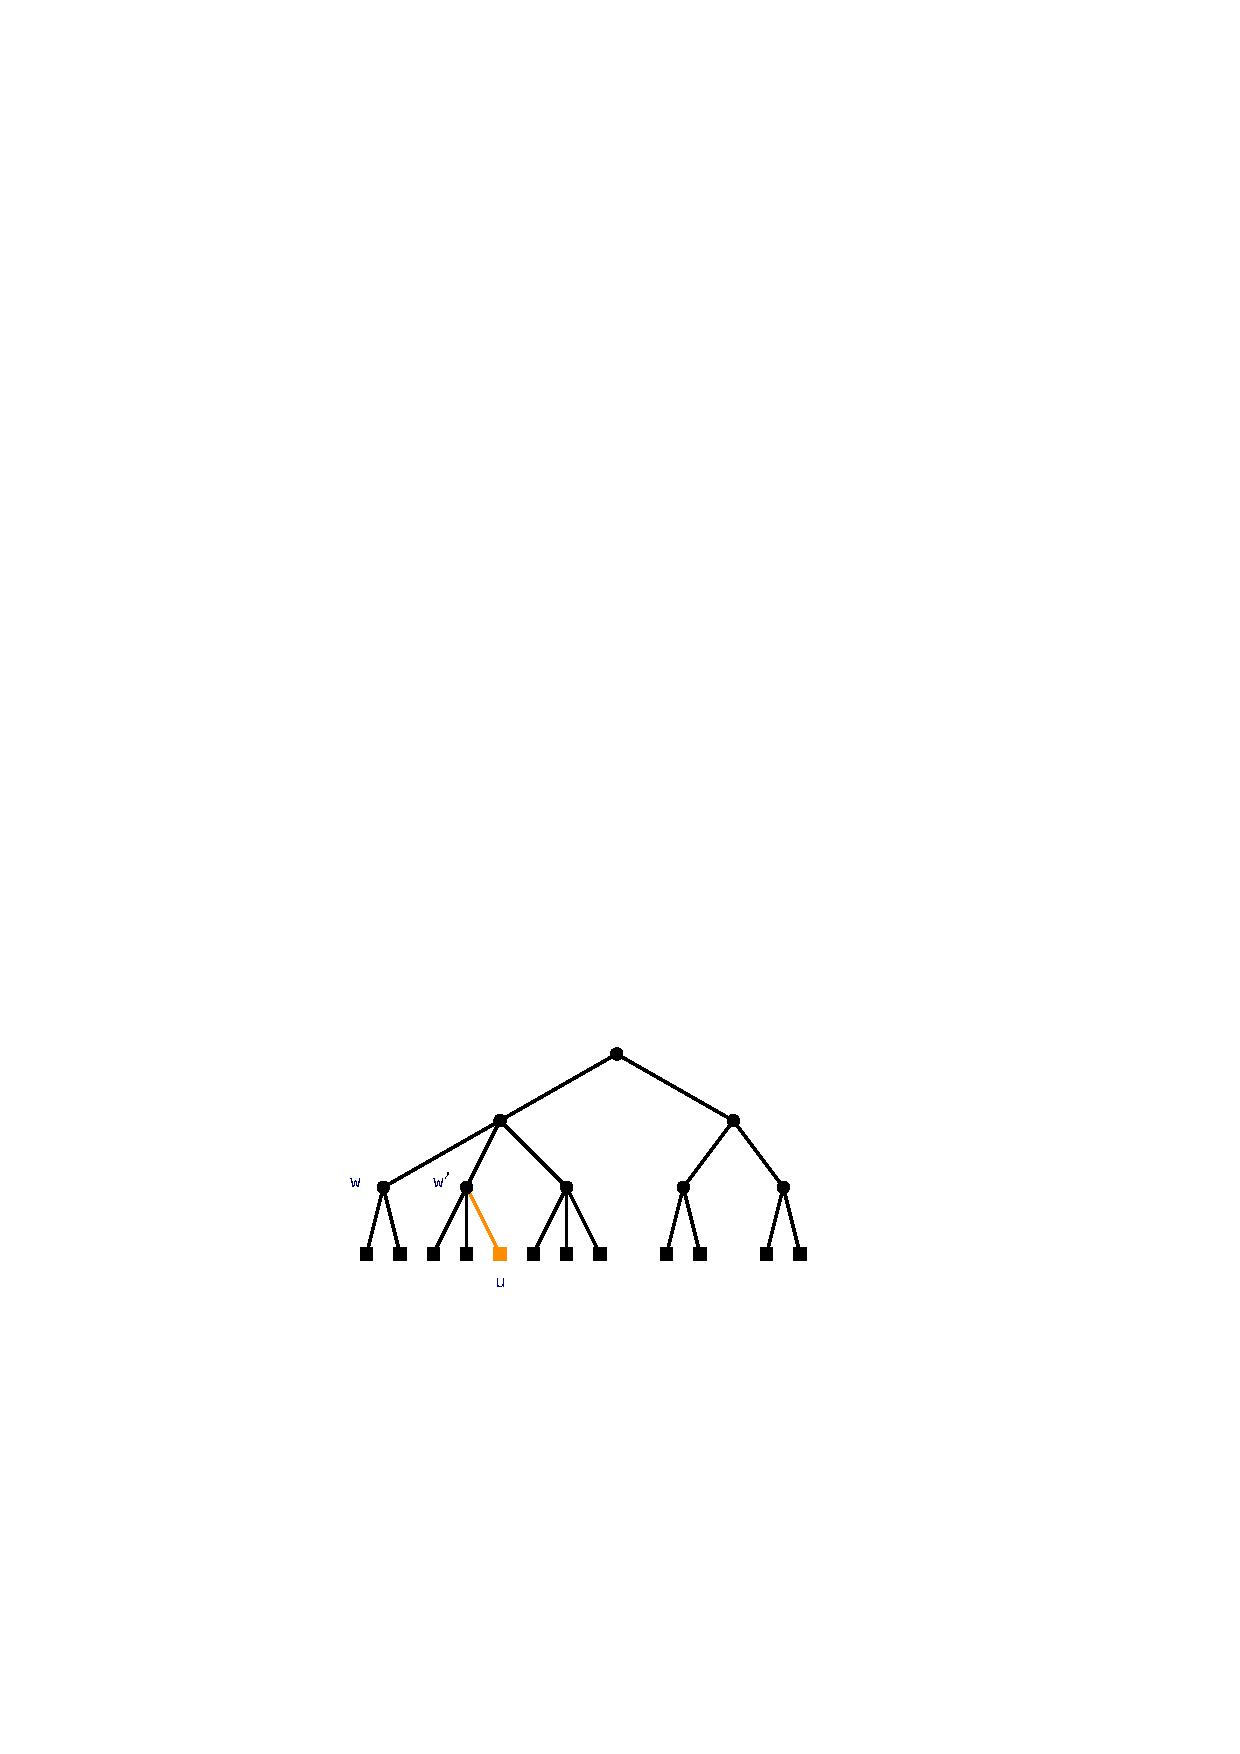
\includegraphics[scale=0.90909]{figs/24tree-add-3}
		\end{tabular}
	\end{center}
	\caption[Adicionando uma folha na árvore 2-4]{Adicionando uma folha na árvore 2-4.
		Este processo termina depois de uma divisão porque #w.parent# tem um grau inferior 
		a 4 antes da adição.}
	\figlabel{twofour-add}
\end{figure}

Uma vez que a altura da árvore 2-4 nunca é maior que $\log #n#$, o
processo de adicionar uma folha termina após $\log #n#$ passos, no máximo.

\subsection{Removendo uma folha}

Remover uma folha da árvore 2-4 é um pouco mais complicado (veja
\figref{twofour-remove}). Para remover uma folha #u# do seu pai #w#, apenas o 
removemos. Se #w# tivesse apenas dois filhos antes da remoção de #u#,
então #w# seria deixado com apenas um filho e violaria a propriedade do grau.

\begin{figure}
	\begin{center}
		\begin{tabular}{c}
			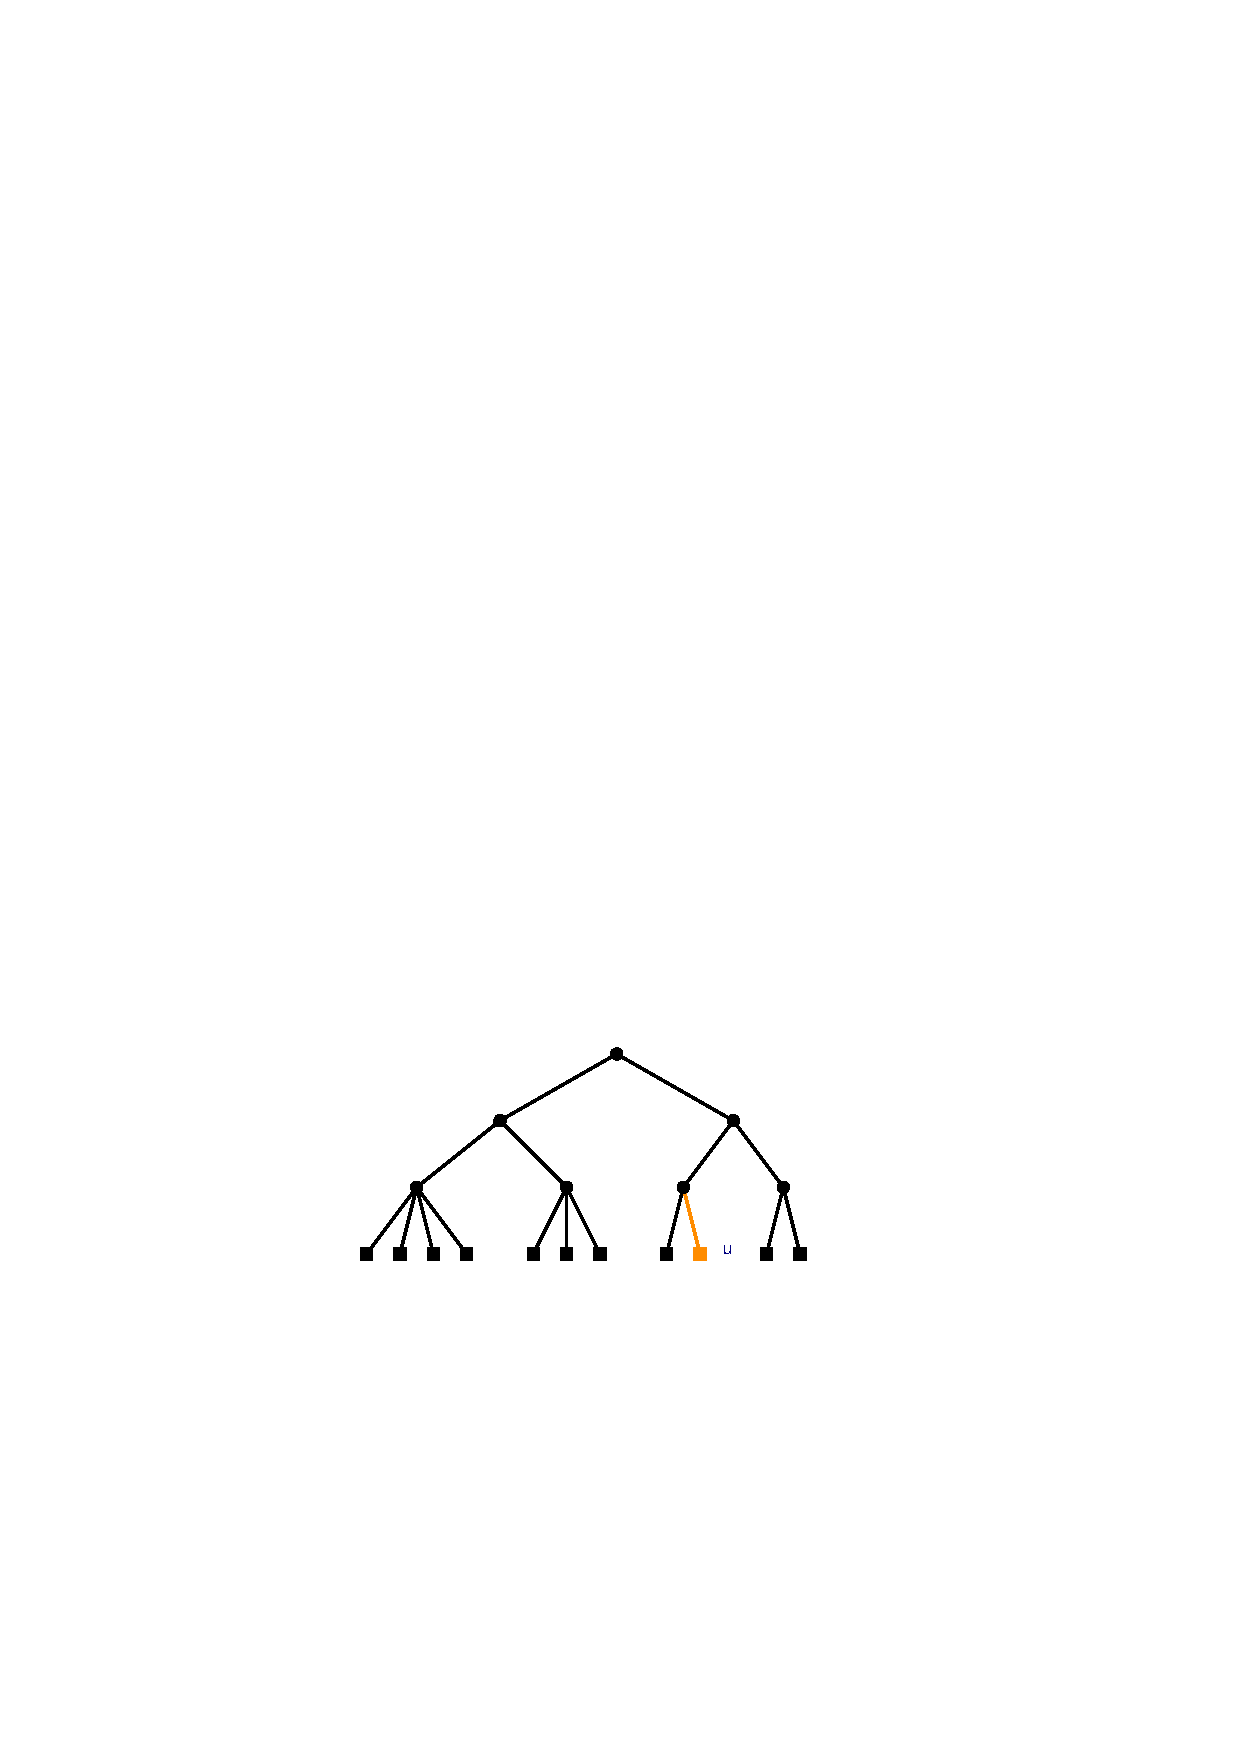
\includegraphics[height=\FifthHeightScaleIfNeeded]{figs/24tree-remove-1} \\
			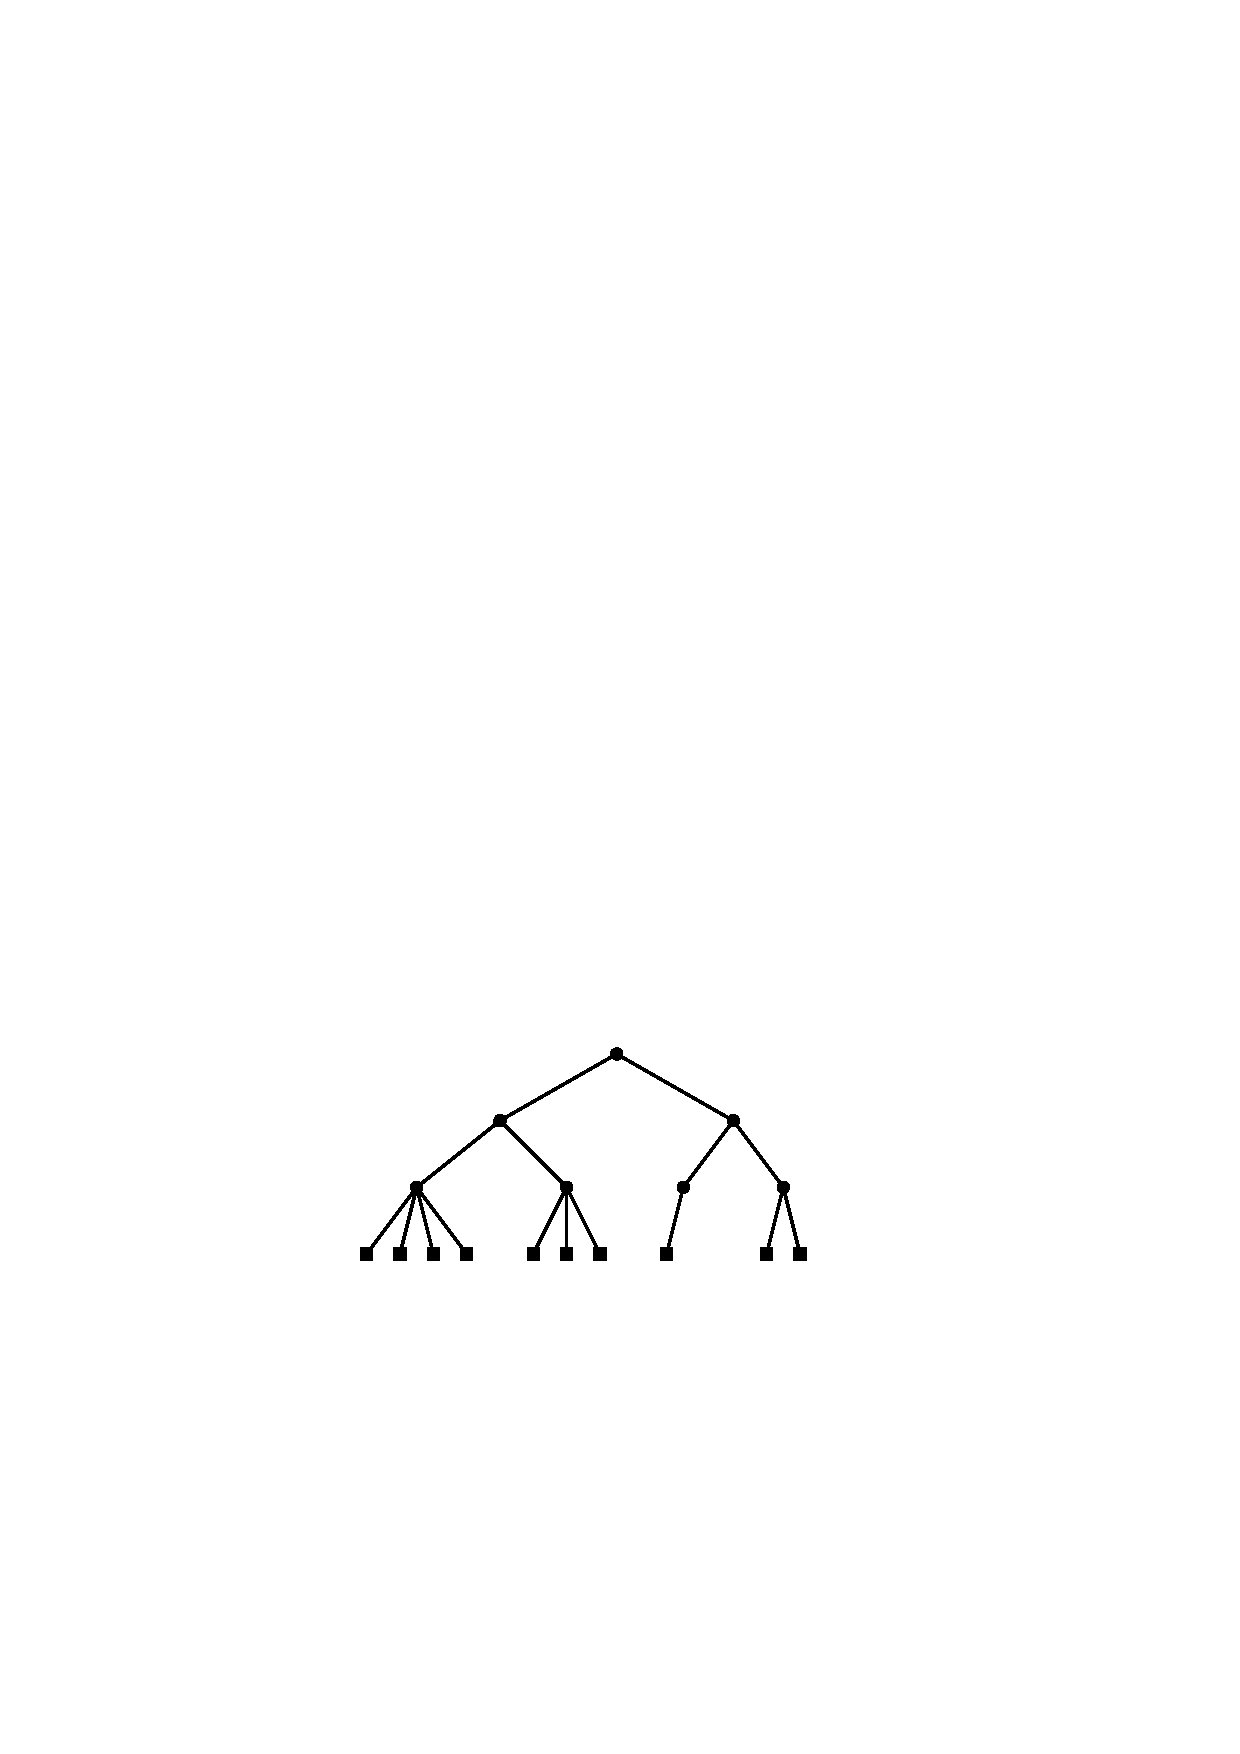
\includegraphics[height=\FifthHeightScaleIfNeeded]{figs/24tree-remove-2} \\
			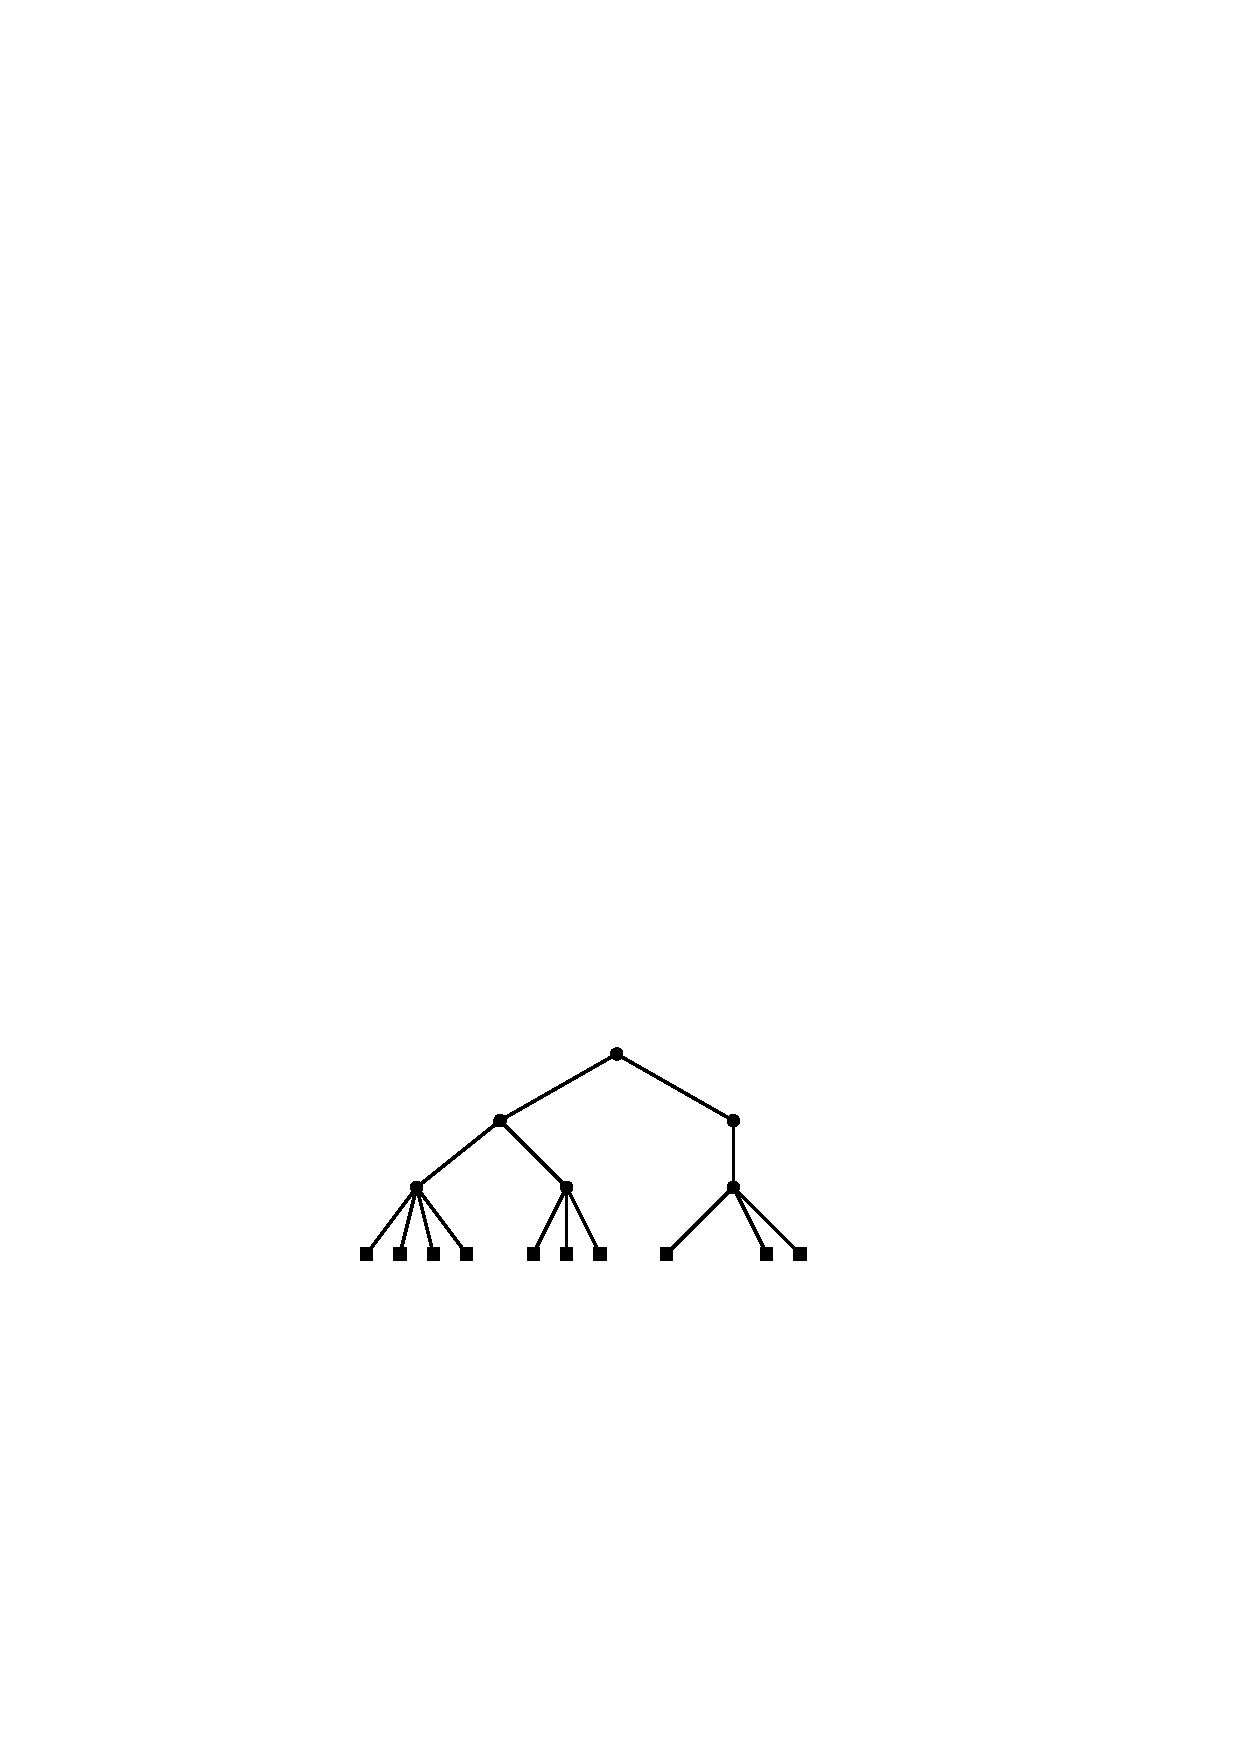
\includegraphics[height=\FifthHeightScaleIfNeeded]{figs/24tree-remove-3} \\
			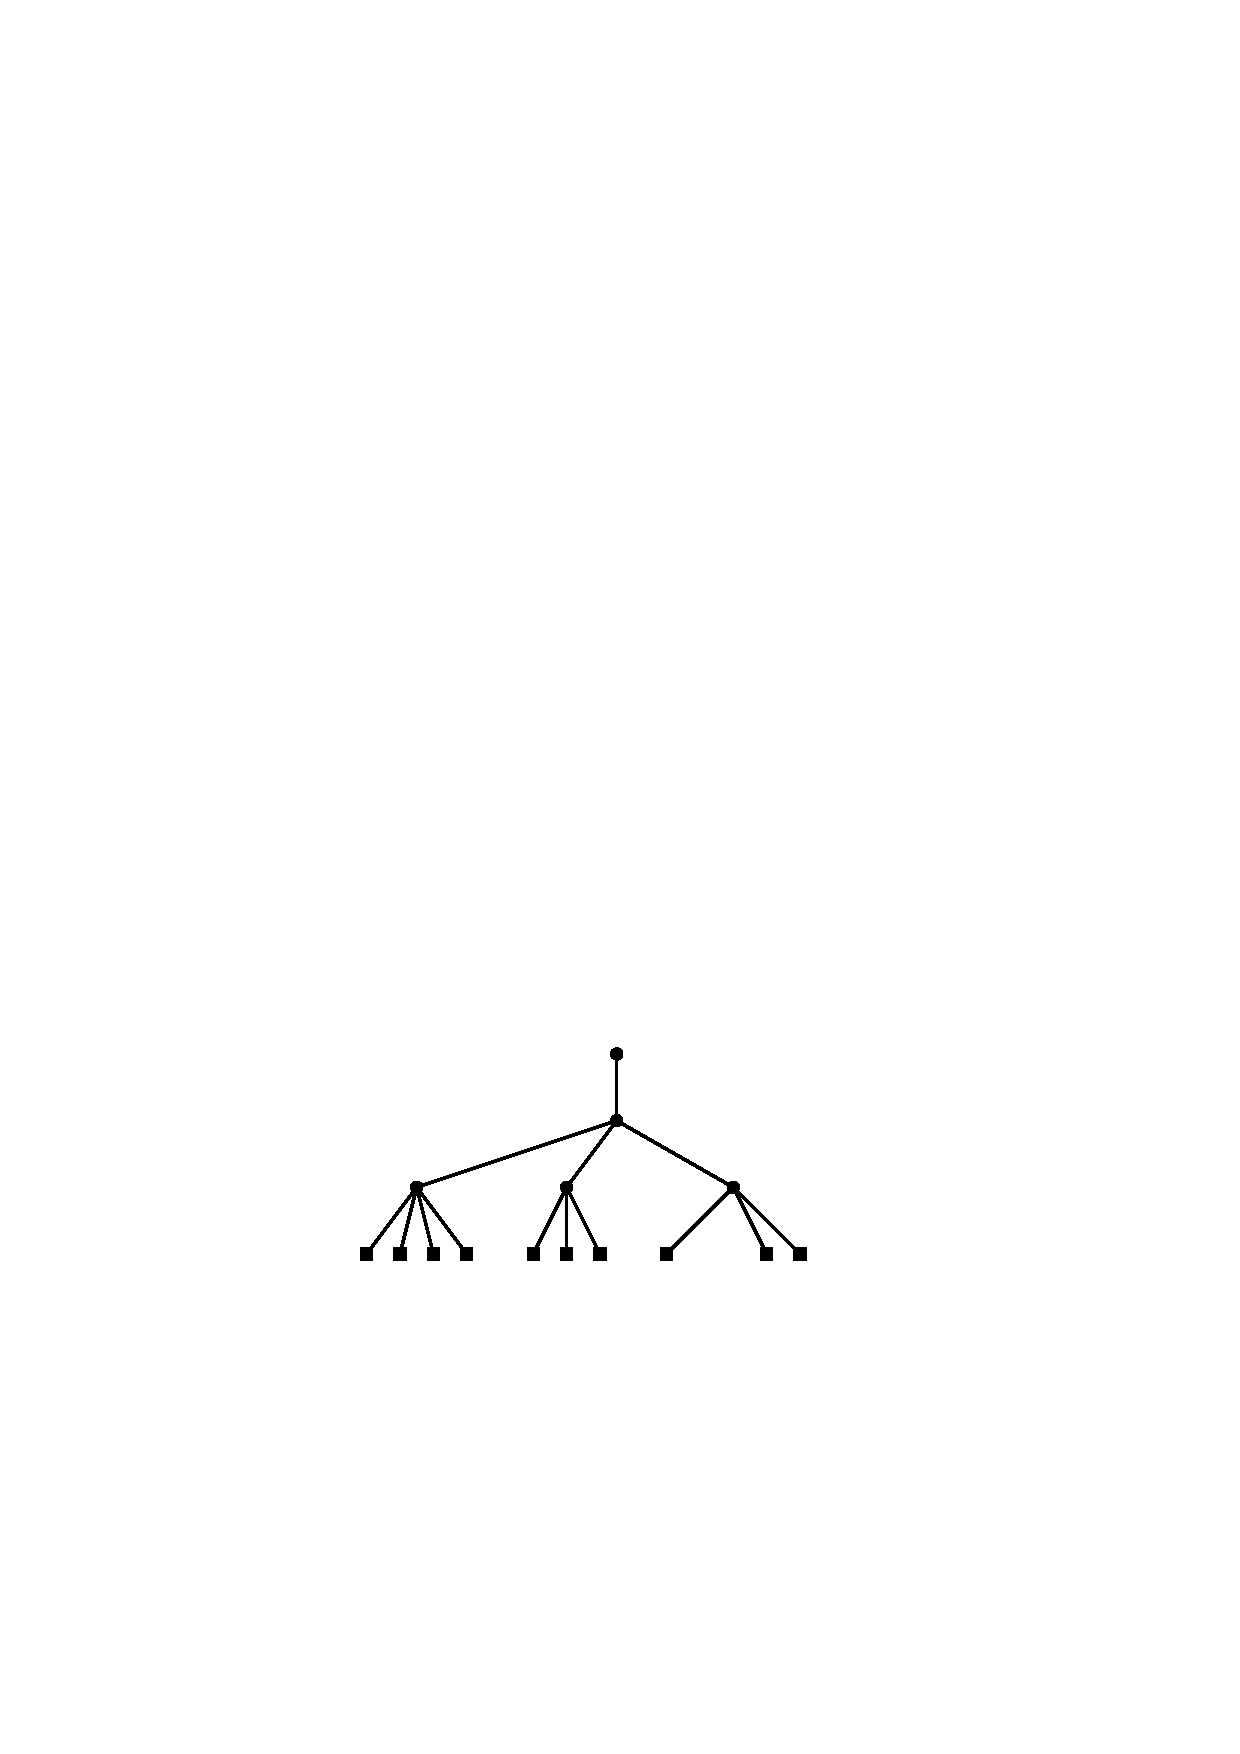
\includegraphics[height=\FifthHeightScaleIfNeeded]{figs/24tree-remove-4} \\
			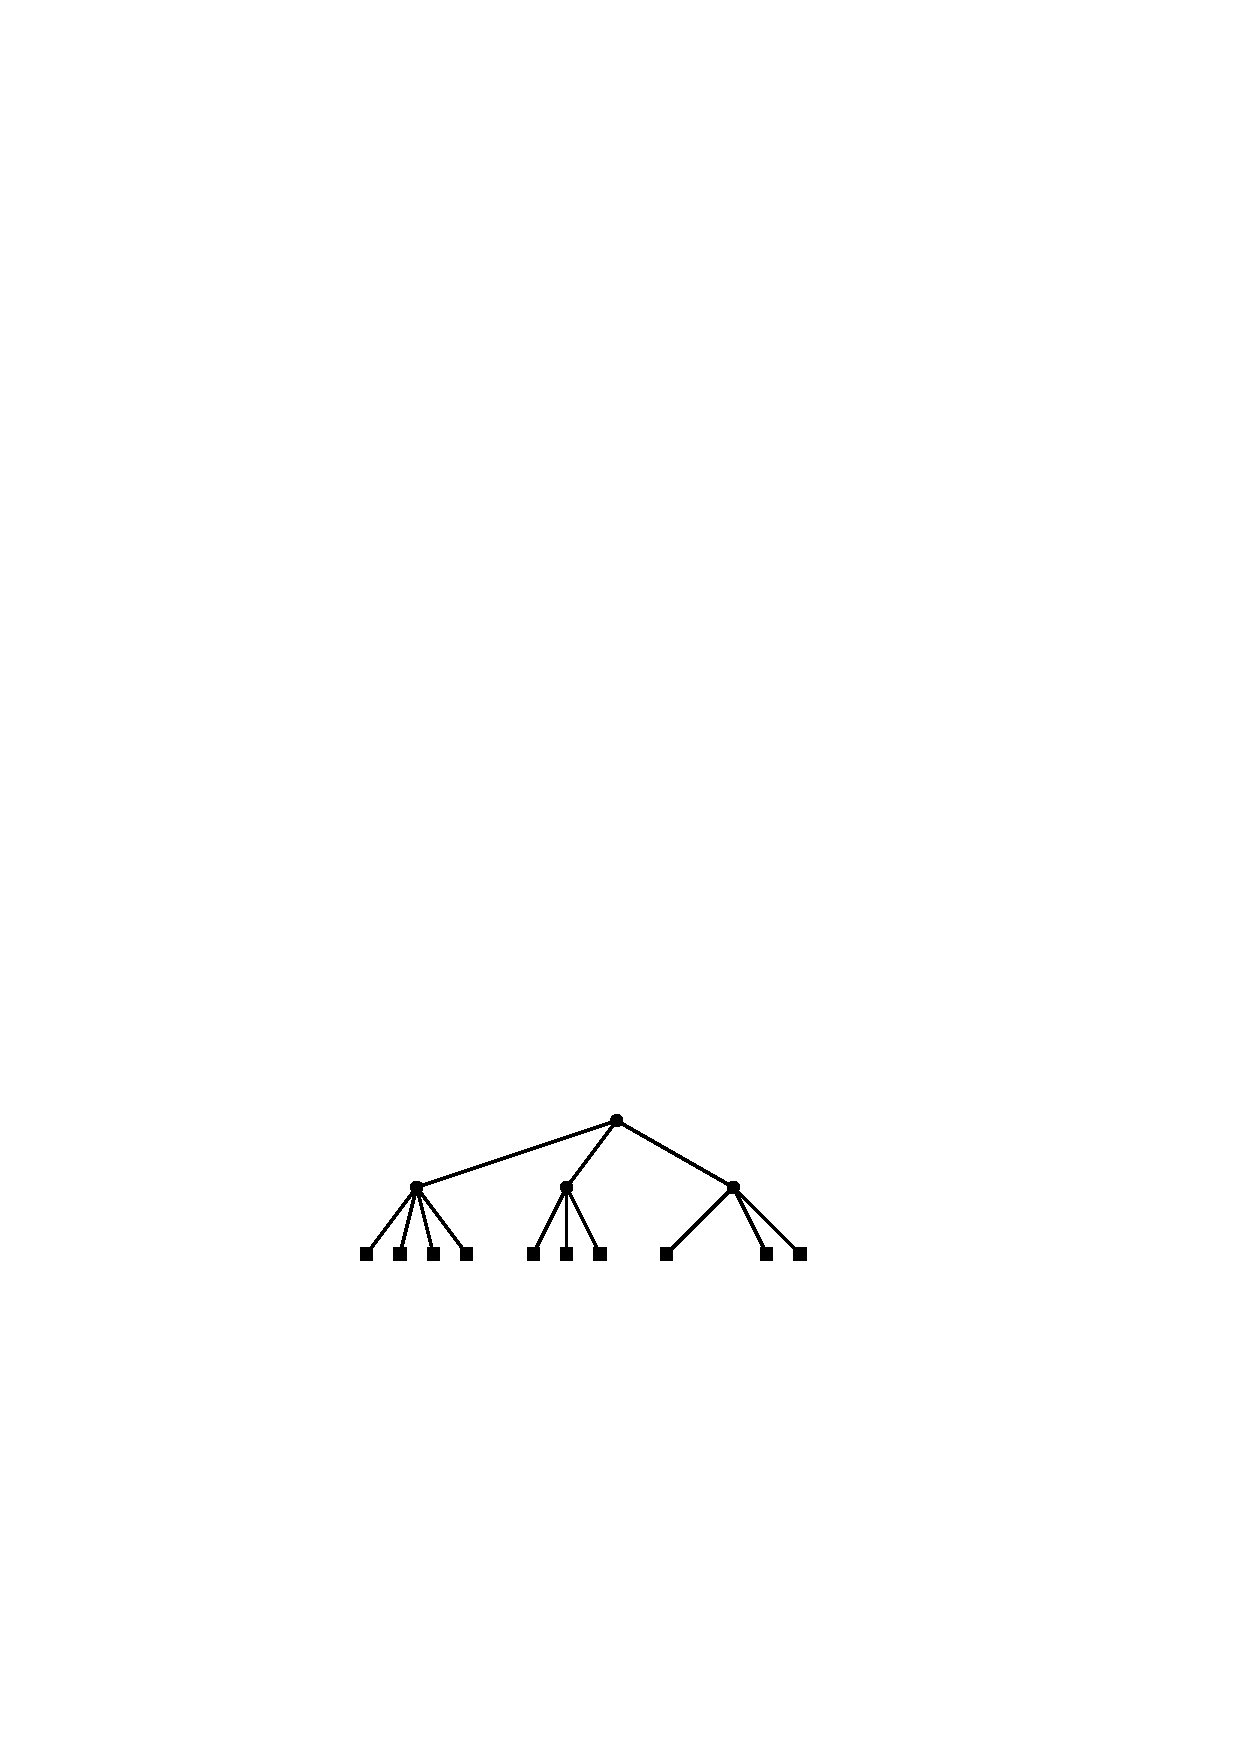
\includegraphics[height=\FifthHeightScaleIfNeeded]{figs/24tree-remove-5} \\
		\end{tabular}
	\end{center}
	\caption[Removing a leaf from a 2-4 Tree]{Removendo uma folha de uma árvore
		2-4.  Este processo vai até a raiz porque cada um dos
		antecessores #u#  e seus irmãos têm somente dois filhos.}
	\figlabel{twofour-remove}
\end{figure}

Para corrigir isso, olhamos para o irmão de #w#, # w' #. O nó #w'# certamente
existe, dado que o pai de #w# tenha pelo menos dois filhos. Se #w'#
tem três ou quatro filhos, então nós levamos um desses filhos de #w'#
para #w#. Agora #w# tem dois filhos, #w'# tem dois ou três
filhos e assim terminamos.

Por outro lado, se #w'# tiver apenas dois filhos, então nós \emph{mesclamos}
\index{merge}%
#w# e #w'# em um único nó, #w#, que tem três filhos. Em seguida,
removemos #w'# do pai de #w'# recursivamente. Esse processo acaba
quando alcançamos um nó, #u#, onde #u# ou seu irmão tem mais de dois
filhos, ou quando chegamos à raiz. No último caso, se a raiz
é deixada com apenas um filho, então nós excluímos a raiz e fazemos do seu filho
a nova raiz. Mais uma vez, isso diminui simultaneamente a altura de cada
folha e, portanto, mantém a propriedade de altura.

Novamente, uma vez que a altura da árvore nunca é mais de $\log #n#$,
o processo de remoção de uma folha termina após um máximo de $\log #n#$ passos.

\section{Árvore Rubro-Negra: Uma Árvore 2-4 Simulada}
\seclabel{redblacktree}

Uma árvore rubro-negra é uma árvore binária de busca na qual
cada nó, #u#, tem uma \emph{cor}
\index{colour}%
que é \emph{vermelha} or \emph{preta}. O vermelho é
representado pelo valor $0$ e preto pelo valor $1$.
\index{red node}%
\index{black node}%
\javaimport{ods/RedBlackTree.red.black.Node<T>}
\cppimport{ods/RedBlackTree.RedBlackNode.red.black}

Antes e depois de qualquer operação em uma árvore rubro-negra, as duas seguintes
propriedades são satisfeitas. Cada propriedade é definida tanto em termos de
cores vermelhas e pretas, como em termos dos valores numéricos 0 e 1.
\begin{prp}[altura preta]
	\index{black-height property}%
	Há o mesmo número de nós pretos em cada caminho da raiz para a folha.
	(A soma das cores em qualquer caminho da raiz para a folha é a mesma.)
\end{prp}

\begin{prp}[sem-borda-vermelha]
	\index{no-red-edge property}%
	Dois nós vermelhos nunca são adjacentes. (Para qualquer nó #u#, exceto a raiz,
	$#u.colour# + #u.parent.colour# \ge 1$.)
\end{prp}
Observe que sempre podemos colorir a raiz, #r#, de uma árvore rubro-negra
sem violar nenhuma dessas duas propriedades, então assumiremos
que a raiz é preta, e os algoritmos para atualizar uma árvore rubro-negra 
irão manter isso. Outro truque que simplifica a árvore rubro-negra
é tratar os nós externos (representados por #nil#) como nós pretos.
Desta forma, todo nó real, #u#, de uma árvore rubro-negra tem exatamente dois
filhos, cada uma com uma cor bem definida. Um exemplo de árvore rubro-negra 
é mostrado em \figref{redblack-example}.

\begin{figure}
	\begin{center}
		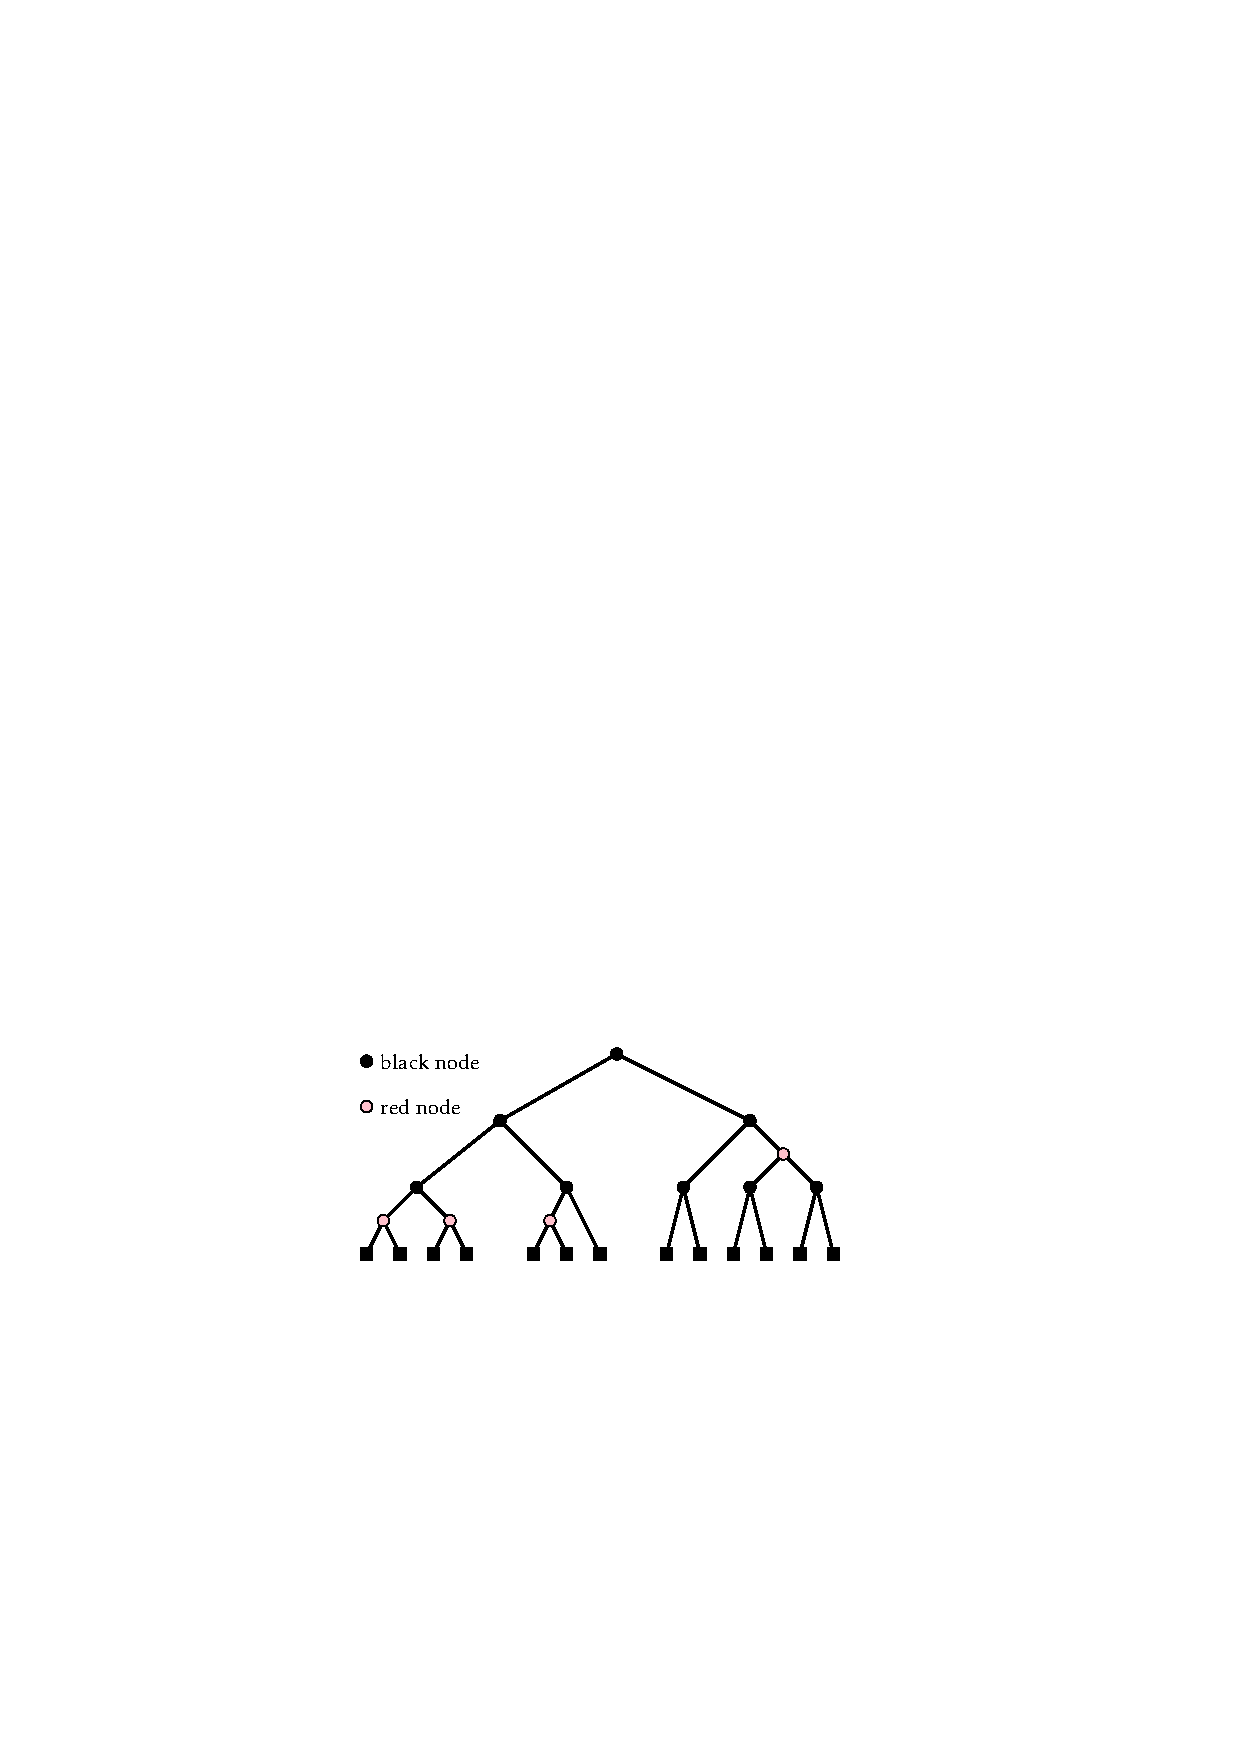
\includegraphics[scale=0.90909]{figs/24rb-1}
	\end{center}
	\caption[A red-black tree]{Um exemplo de uma árvore rubro-negra com altura preta 3. Os nós externos (#nil#) são desenhados como quadrados.}
	\figlabel{redblack-example}
\end{figure}


\subsection{Árvores Rubro-Negras e Árvores 2-4}

No começo, pode parecer surpreendente que uma árvore rubro-negra possa ser eficientemente
atualizada para manter as propriedades altura-preta e sem-borda-vermelha, e
parece incomum mesmo considerar estas como propriedades úteis. Contudo,
árvores rubro-negras foram projetadas para ser uma simulação eficiente de árvores 2-4
como árvores binárias.

Consulte a \figref{twofour-redblack}.
Considere qualquer árvore rubro-negra, $T$, tendo #n# nós e executando a
seguinte transformação: remova cada nó vermelho #u# e conecte os dois
filhos de #u# diretamente ao pai (preto) de #u#. Após essa transformação
nós ficamos com uma árvore $T'$ tendo apenas nós pretos.
\begin{figure}
	\begin{center}
		\begin{tabular}{cc}
			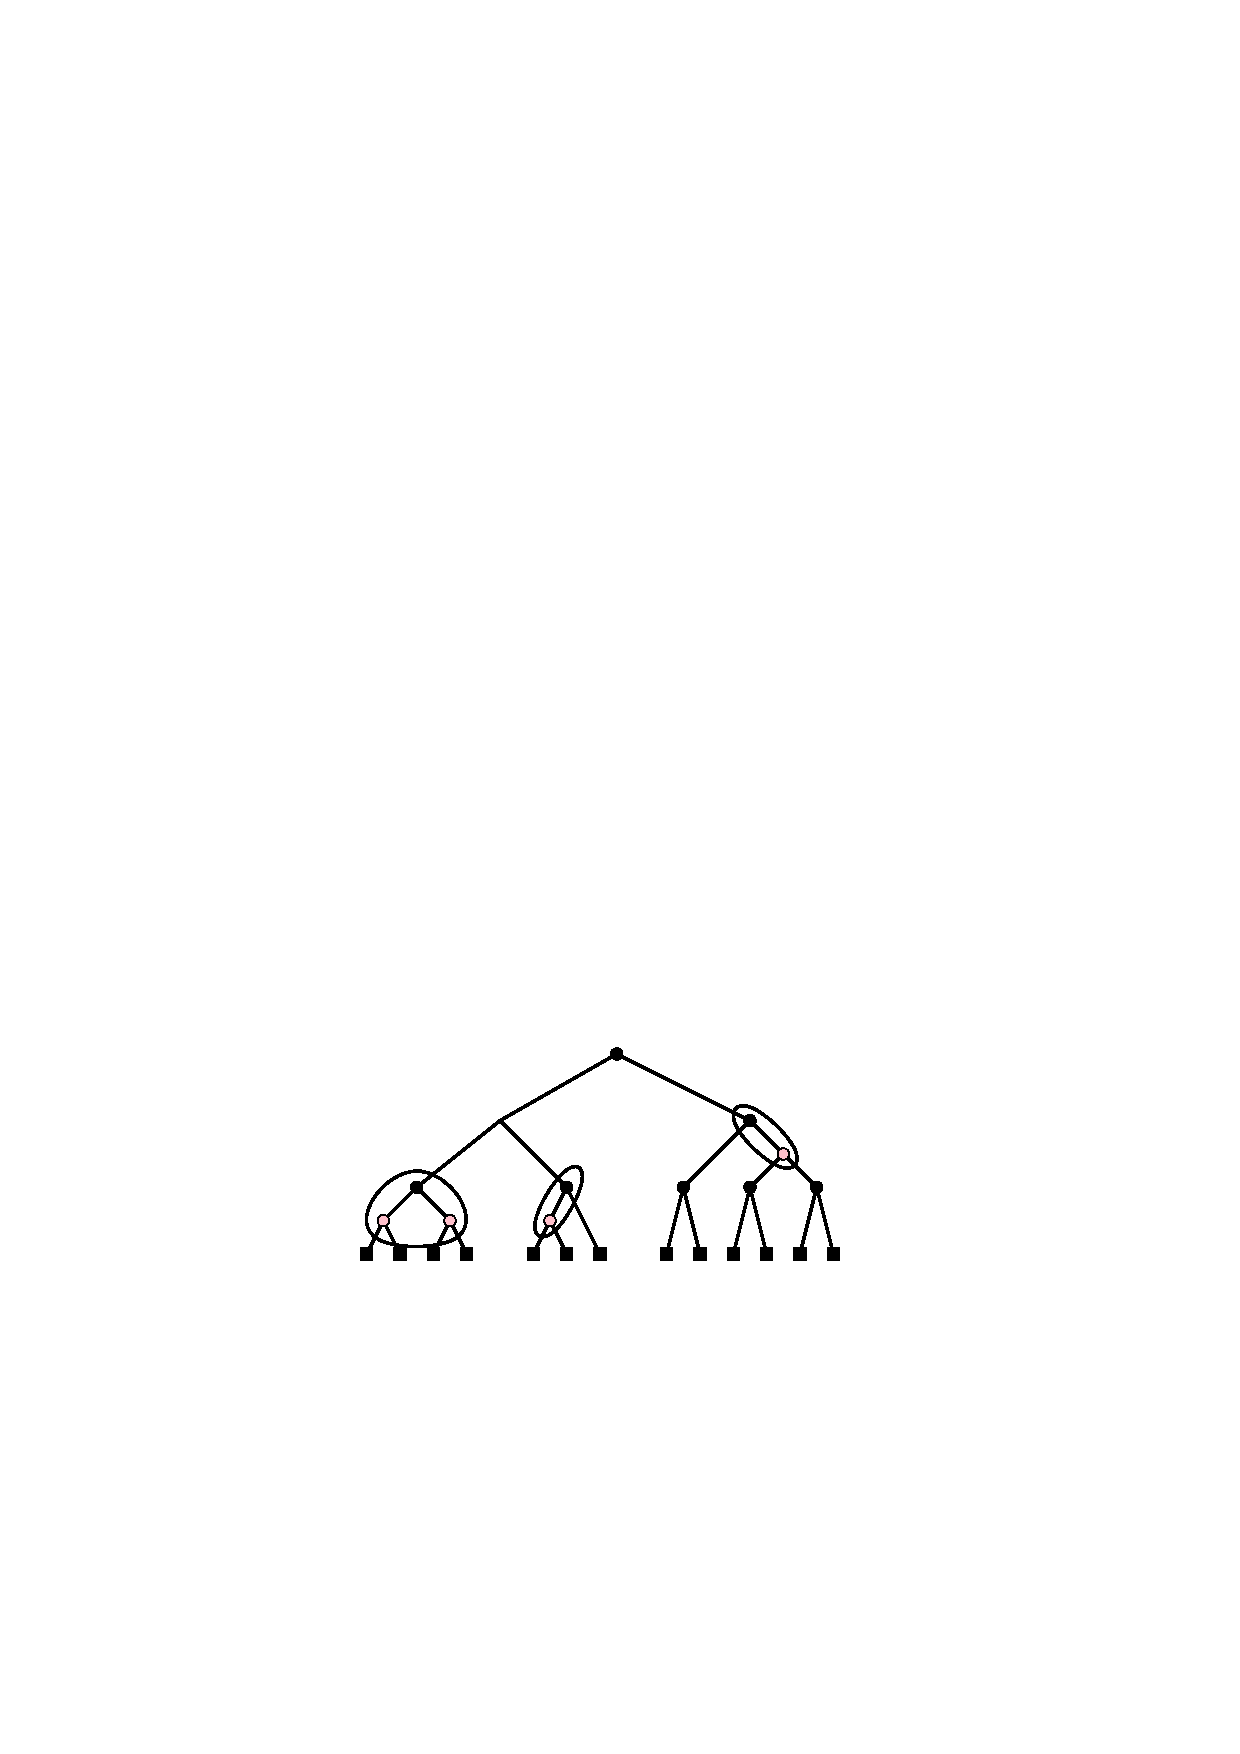
\includegraphics[scale=0.90909]{figs/24rb-3} \\
			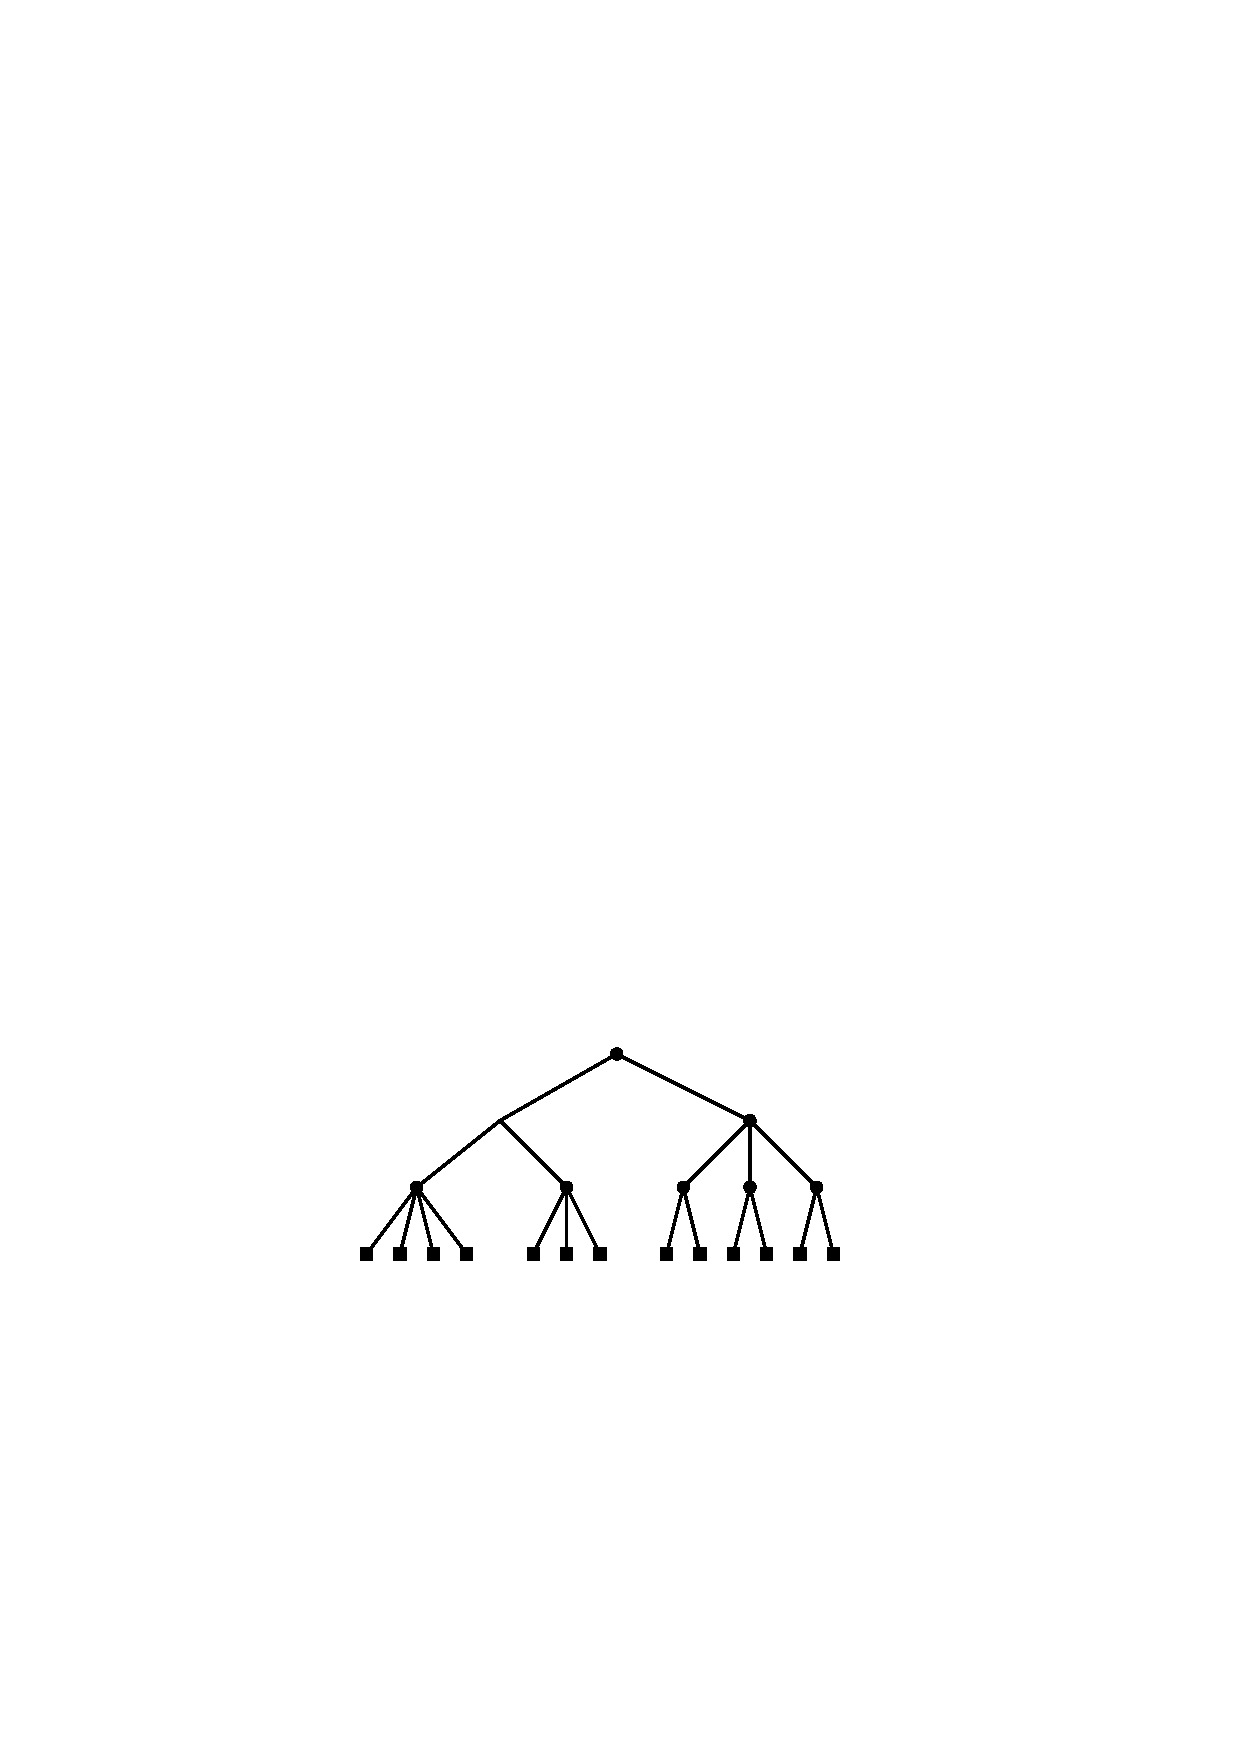
\includegraphics[scale=0.90909]{figs/24rb-2}
		\end{tabular}
	\end{center}
	\caption{Toda árvore rubro-negra possui uma árvore 2-4 correspondente.}
	\figlabel{twofour-redblack}
\end{figure}

Cada nó interno em $T'$ tem dois, três ou quatro filhos: Um nó preto
que começou com dois filhos pretos ainda terá dois
filhos pretos após essa transformação. Um nó preto que começou
com um filho vermelho e um preto terá três filhos depois dessa
transformação. Um nó preto que começou com dois filhos vermelhos
terá quatro filhos após essa transformação. Além disso, a
propriedade altura-preta agora garante que cada caminho da raiz até a folha em $T'$ tem o
mesmo comprimento. Em outras palavras, $T'$ é uma árvore 2-4!

A árvore 2-4 $T'$ tem $ #n#+1$ folhas que correspondem aos $#n#+1$
nós externos da árvore rubro-negra. Portanto, esta árvore tem, no máximo, altura
$\log (#n#+1)$. Agora, cada caminho da raiz até a folha na árvore 2-4 corresponde
a uma rota da raiz da árvore rubro-negra $T$ até um nó externo.
O primeiro e último nó neste caminho são pretos, e no máximo um, a
cada dois nós internos, é vermelho. Então esta rota tem no máximo $\log(#n#+1)$
nós pretos e no máximo $\log(#n#+1)-1$ nós vermelhos. Portanto, a rota mais longa da raiz para qualquer nó \emph{interno} em $T$ é no máximo
\[
2\log(#n#+1) -2 \le 2\log #n# \enspace ,
\]
para qualquer $#n#\ge 1$. Isso prova a propriedade mais importante da
árvore rubro-negra:
\begin{lem}
	A altura da árvore rubro-negra com #n# nós é no máximo $2\log #n#$.
\end{lem}

Agora que vimos a relação entre árvores 2-4  e
árvores rubro-negras, não é difícil acreditar que podemos manter,
eficientemente, uma árvore rubro-negra ao adicionar e remover elementos.

Já vimos que adicionar um elemento em uma \textit{Árvore Binária de Busca}
pode ser feito adicionando uma nova folha. Portanto, para implementar #add(x)# em uma
árvore rubro-negra, precisamos de um método para simular a divisão de um nó com cinco
filhos em uma árvore 2-4. Um nó de árvore 2-4 com cinco filhos é representado
por um nó preto que tem dois filhos vermelhos, um dos quais também tem um filho
vermelho. Nós podemos dividir esse nó colorindo-o de vermelho e colorindo
dois filhos pretos. Um exemplo disso é mostrado em \figref{rb-split}.

\begin{figure}
	\begin{center}
		\begin{tabular}{c}
			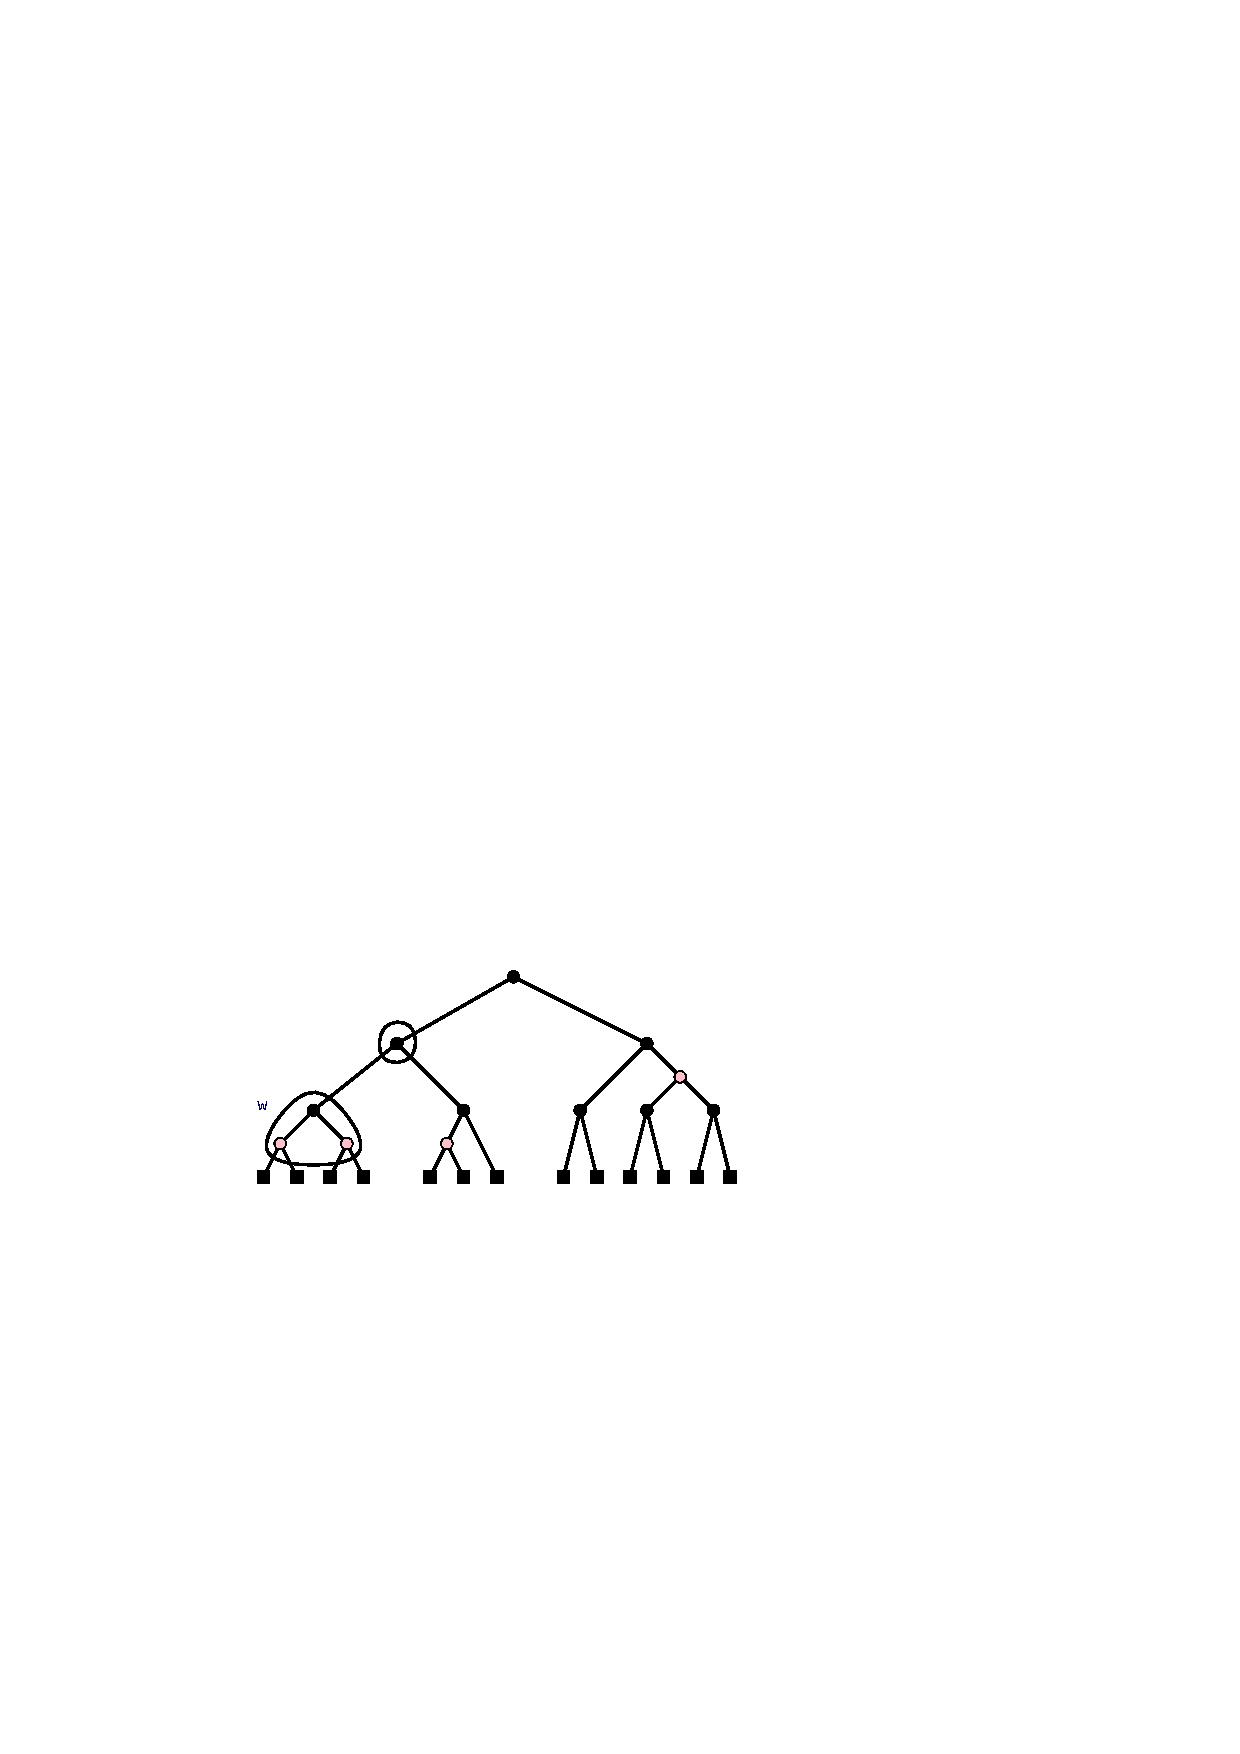
\includegraphics[scale=0.90909]{figs/rb-split-1} \\
			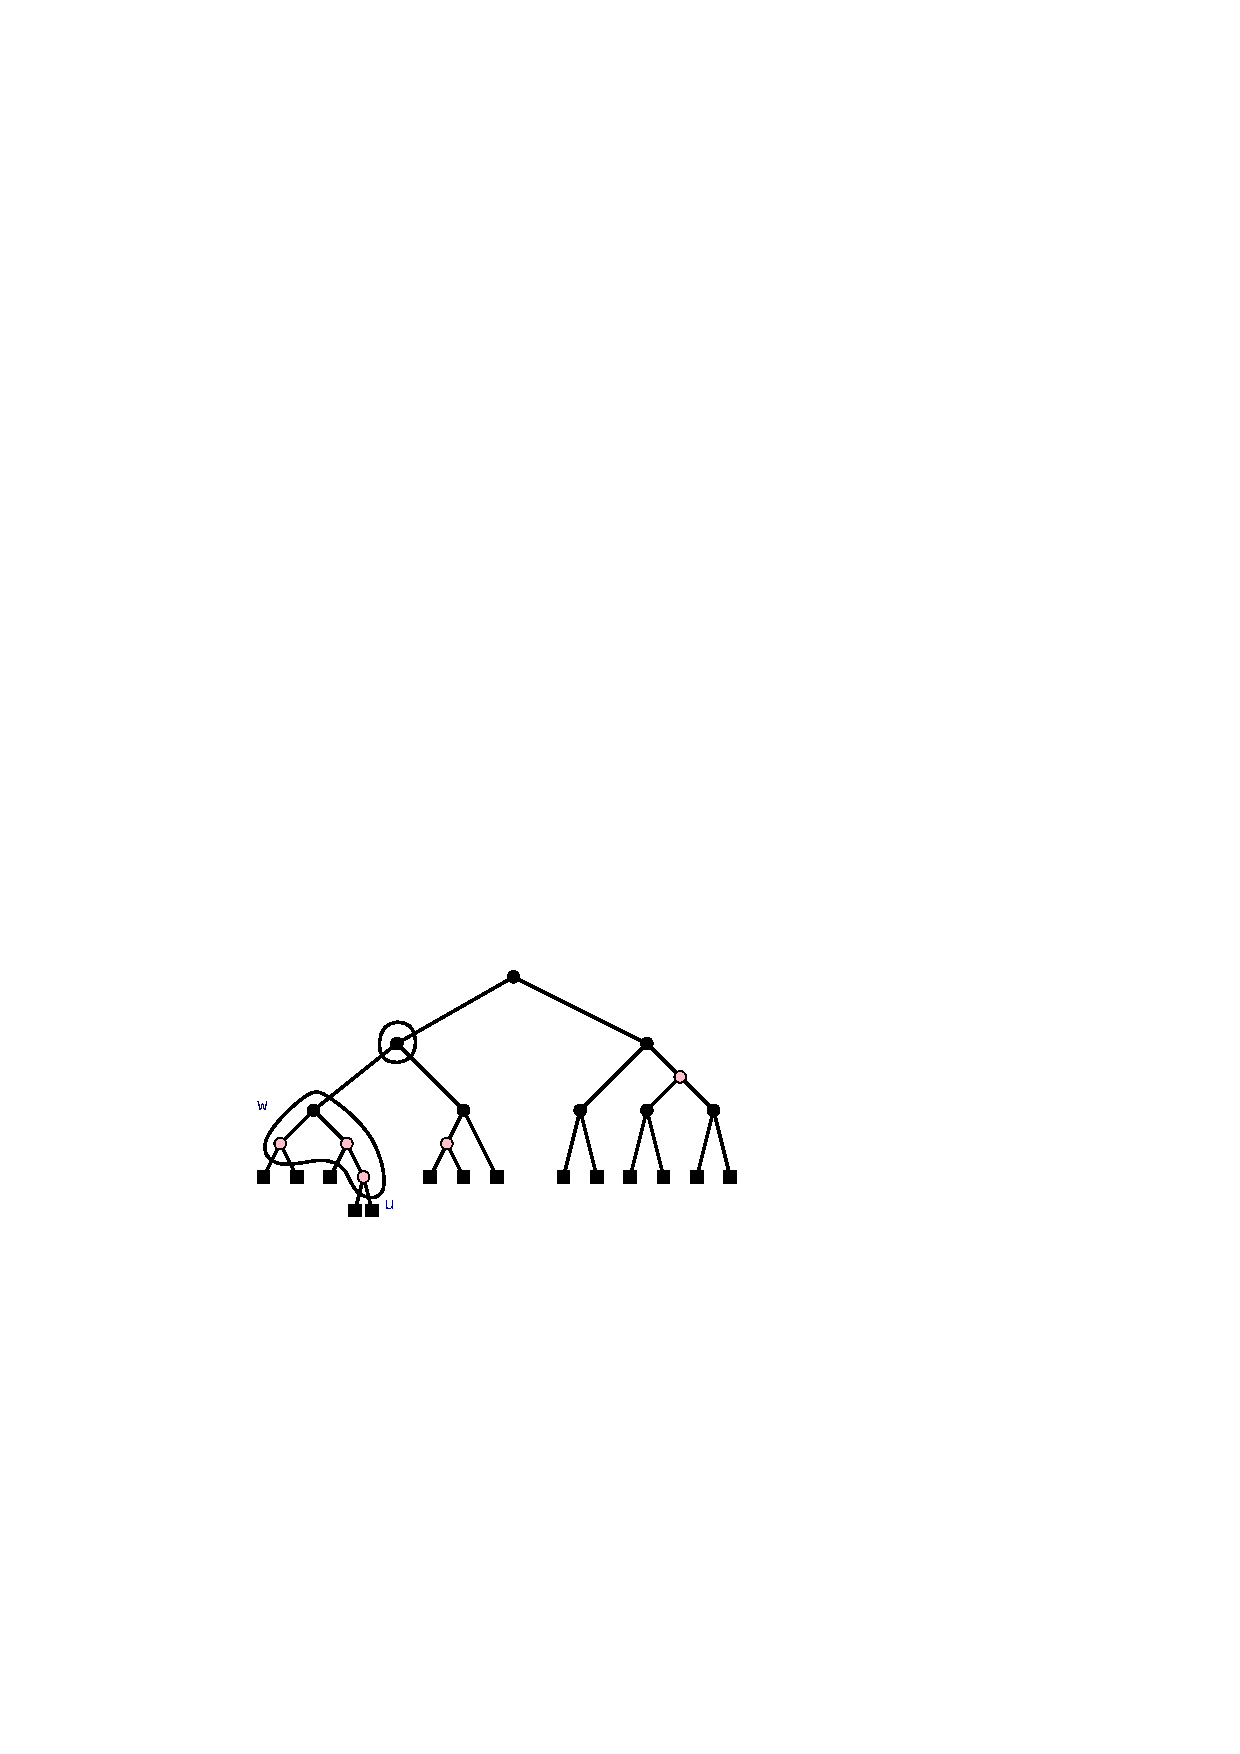
\includegraphics[scale=0.90909]{figs/rb-split-2} \\
			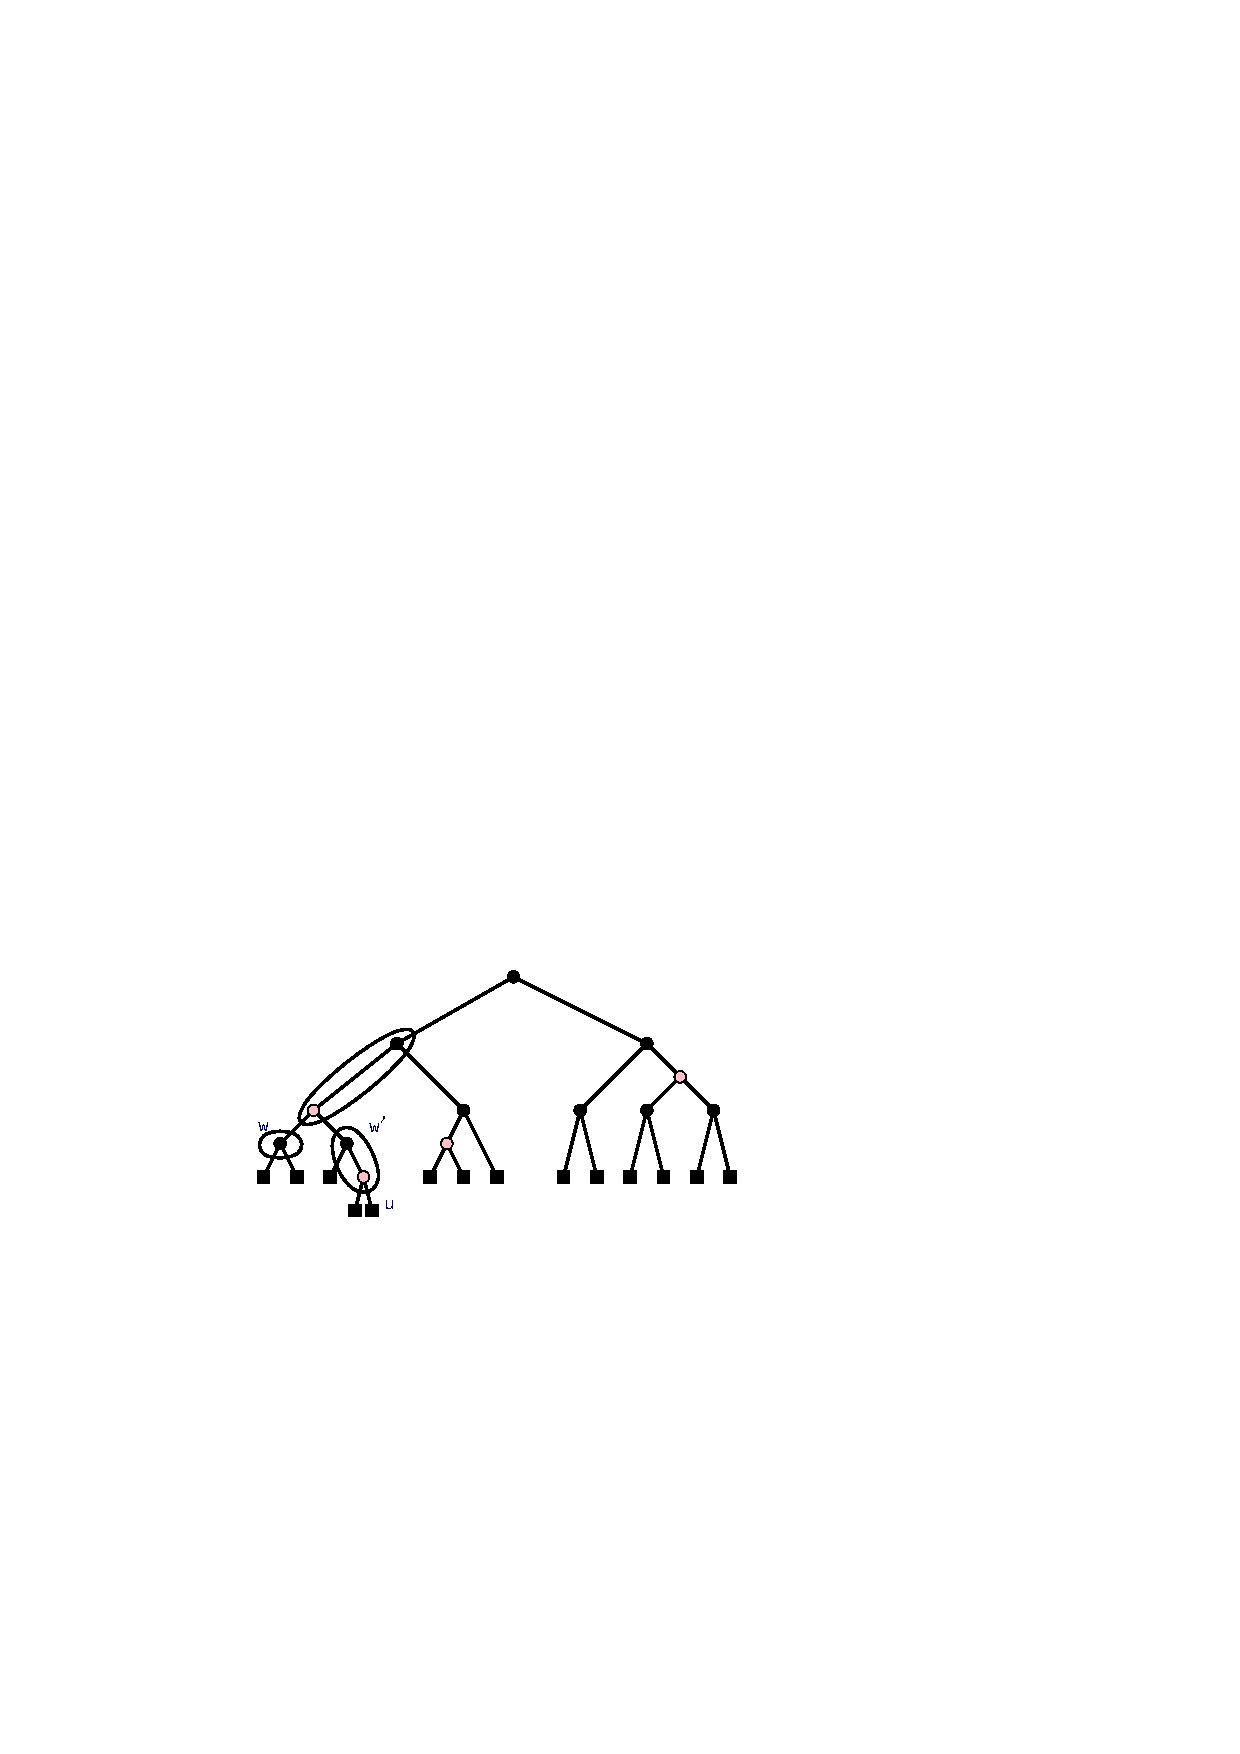
\includegraphics[scale=0.90909]{figs/rb-split-3} \\
		\end{tabular}
	\end{center}
	\caption[Simulando uma árvore 2-4] {Simulando uma operação de divisão em árvore 2-4
		durante uma adição em uma árvore rubro-negra. (Isto simula a adição em
		árvore 2-4 mostrada em \figref{twofour-add}.)}
	\figlabel{rb-split}
\end{figure}

Da mesma forma, implementar o método #remove(x)# requer um método de mesclagem 
de dois nós, e pegar emprestado um filho de um irmão. Mesclar dois nós é o inverso de
uma divisão (mostrado em \figref{rb-split}), e envolve colorir, de vermelho, dois
irmãos pretos e colorir, de preto, o pai vermelho. Pegar emprestado de
um irmão é o procedimento mais complicado e envolve
rotações e recolorações de nó.

Claro, durante todo isso, ainda devemos manter as propriedades sem-borda-vermelha
e altura-preta. Embora não seja mais surpreendente que isso possa ser feito,
há uma grande quantidade de casos que precisam ser considerados se tentarmos 
fazer uma simulação direta de uma árvore 2-4 através de uma
árvore rubro-negra. Em algum momento, torna-se mais simples ignorar a
árvore 2-4 subjacente e trabalhar diretamente para manter as propriedades
da árvore rubro-negra.

\subsection{Árvores Rubro-Negras caindo para a esquerda}

\index{árvore rubro-negra}%
\index{lárvore rubro-negra caindo para a esquerda}%
Não existe uma definição única de árvores rubro-negras. Em vez disso, existe
uma família de estruturas que conseguem manter as propriedades altura-preta
e sem-borda-vermelha durante as operações #add(x)# e #remove(x)#. 
Diferentes estruturas fazem isso de diferentes maneiras.
Aqui, implementamos a estrutura de dados que chamamos de #RedBlackTree#.
\index{RedBlackTree@#RedBlackTree#}%
Esta estrutura implementa uma variante particular das árvores rubro-negras que
satisfaz uma propriedade adicional:
\begin{prp}[left-leaning]\prplabel{left-leaning}\prplabel{redblack-last}
	\index{propriedade caindo para a esquerda}%
	Em qualquer nó #u#, se #u.left# for preto, então #u.right# é preto.
\end{prp}
Observe que a árvore rubro-negra mostrada em \figref{redblack-example} não
satisfaz a propriedade caindo-para-esquerda; ela é violada pelo pai do
nó vermelho no caminho mais à direita.

O motivo para manter a propriedade caindo-para-esquerda é que ela reduz
o número de casos encontrados ao atualizar a árvore durante #add(x)#
e #remove(x)# operações. Em termos de árvores 2-4, isso implica que cada
árvores 2-4 tem uma representação única: um nó de grau dois torna-se
um nó preto com dois filhos pretos. Um nó de grau três torna-se
um nó preto cujo filho esquerdo é vermelho e cujo filho direito é preto.
Um nó de grau quatro torna-se um nó preto com dois filhos vermelhos.

Antes de descrever a implementação de #add (x)# e #remove(x)# em
detalhe, apresentamos algumas sub-rotinas simples usadas por esses métodos
que estão ilustradas na \figref{redblack-flippullpush}. As duas primeiras
sub-rotinas são para manipular cores, preservando a propriedade altura-negra.
O método #pushBlack(u)# recebe como entrada um nó preto #u#
que tem dois filhos vermelhos e então colore #u# de vermelho e seus dois filhos 
de preto. O método #pullBlack(u)# inverte esta operação:
\codeimport{ods/RedBlackTree.pushBlack(u).pullBlack(u)}

\begin{figure}
	\begin{center}
		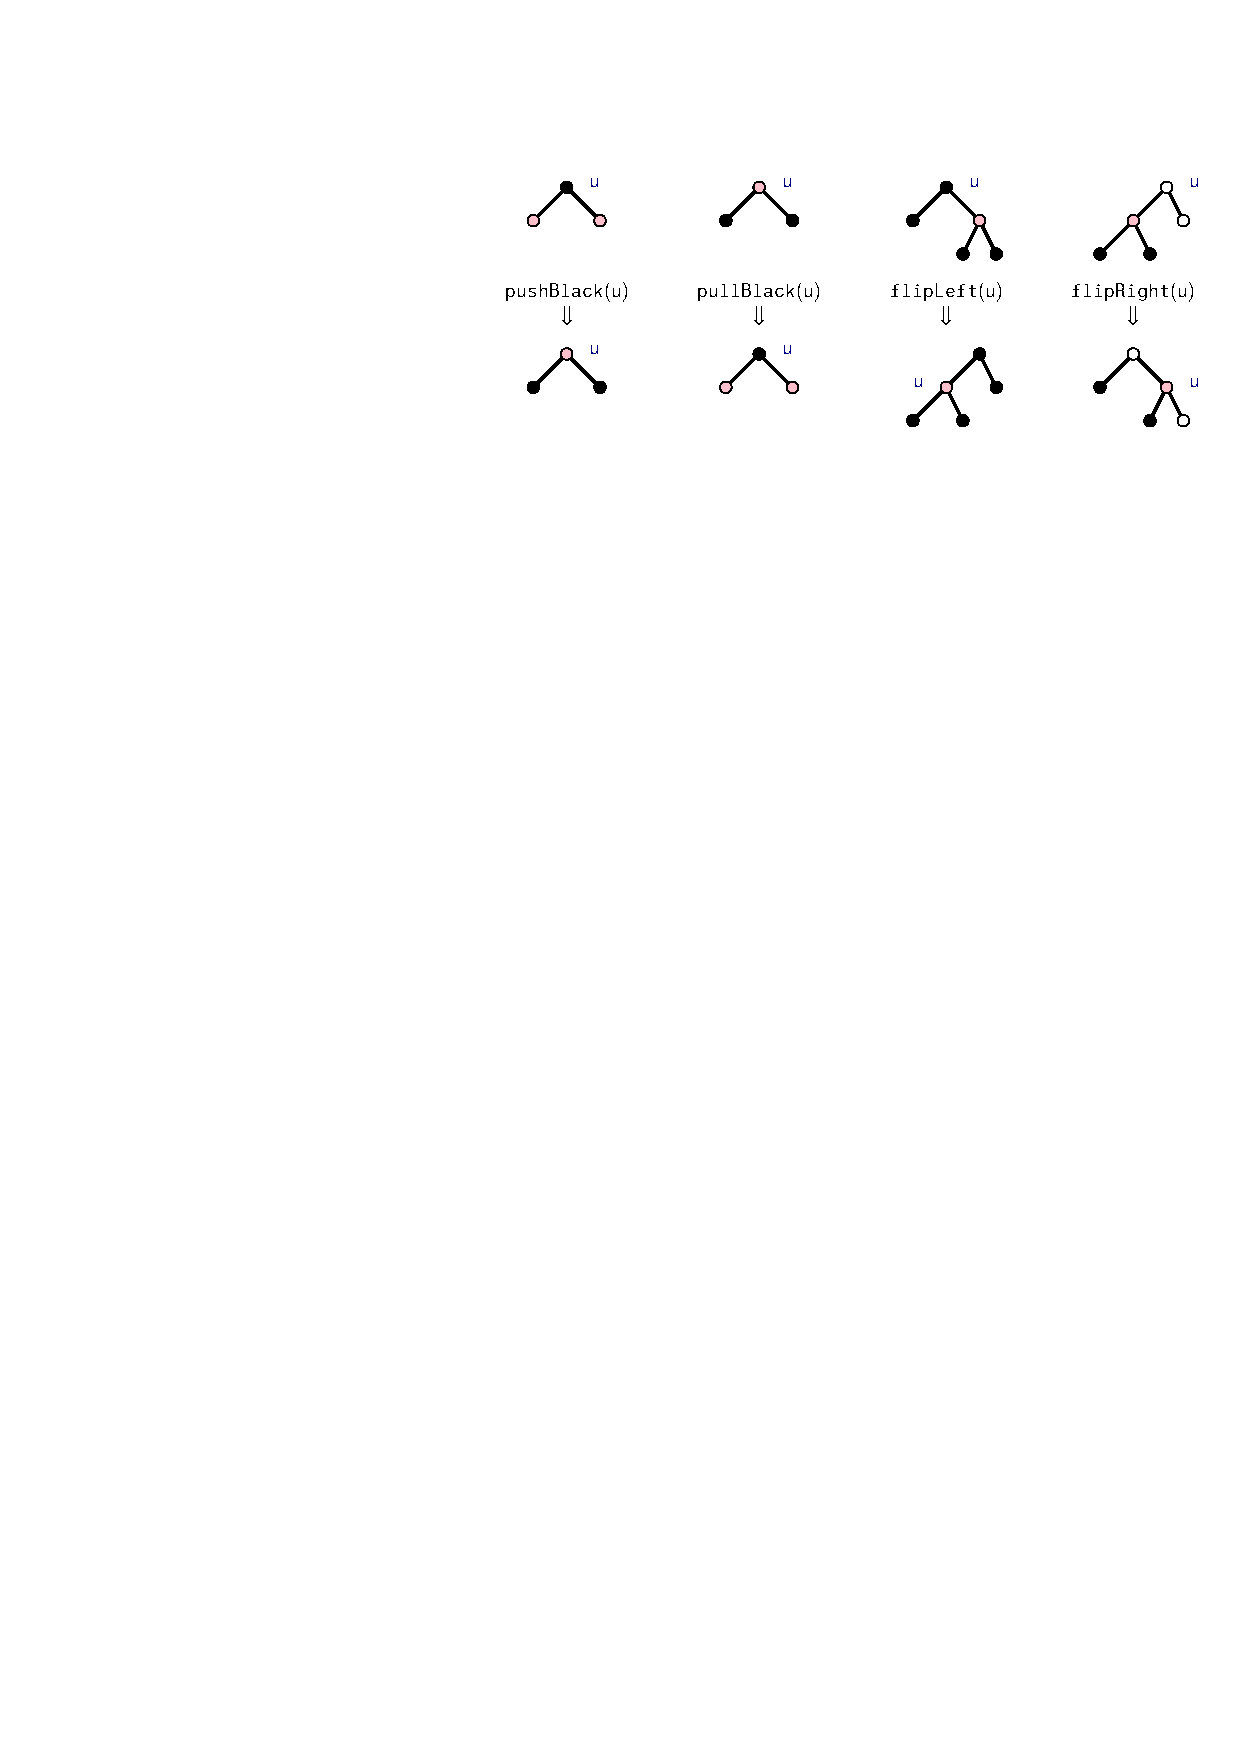
\includegraphics[width=\ScaleIfNeeded]{figs/flippullpush}
	\end{center}
	\caption{Flips, pulls e pushes}
	\figlabel{redblack-flippullpush}
\end{figure}

O método #flipLeft(u)# troca as cores de #u# e #u.right#
e então executa uma rotação à esquerda em #u#. Este método inverte as
cores desses dois nós, bem como sua relação pai-filho:
\codeimport{ods/RedBlackTree.flipLeft(u)}
A operação #flipLeft(u)#
é especialmente útil para restaurar a propriedade caindo-pra-esquerda em um nó
#u# que a viola (porque #u.left# é preto e #u.right# é vermelho).
Neste caso especial, podemos ter certeza de que esta operação preserva ambas
as propriedades altura-preta e sem-borda-vermelha. A operação #flipRight(u)#
é simétrica com #flipLeft(u)#, quando os papéis da esquerda e direita são invertidos.
\codeimport{ods/RedBlackTree.flipRight(u)}

\subsection{Adição}

Para implementar #add(x)# em uma #RedBlackTree#, nós executamos um inserção 
padrão em #BinarySearchTree# para adicionar uma nova folha, #u#, com $#u.x#=#x#$
e definir $#u.colour#=#red#$. Observe que isso não altera a altura preta
de qualquer nó, por isso não viola a propriedade de altura-preta. No entanto, pode
violar a propriedade caindo-para-esquerda (se #u# é o filho direito de
seu pai), e isso pode violar a propriedade sem-borda-vermelha (se o pai de #u#
é #vermelho#). Para restaurar essas propriedades, chamamos o método #addFixup(u)#.
\codeimport{ods/RedBlackTree.add(x)}

Ilustrado em \figref{rb-addfix}, o método #addFixup(u)# recebe como 
entrada um nó #u# cuja cor é o vermelho e que pode violar as 
propriedades sem-borda-vermelha e/ou caindo-para-esquerda. A seguinte 
discussão é provavelmente impossível de se explicar sem se referir a
\figref{rb-addfix} ou recriá-la em um pedaço de papel. De fato, o
leitor talvez deseje estudar essa figura antes de continuar.

\begin{figure}
	\begin{center}
		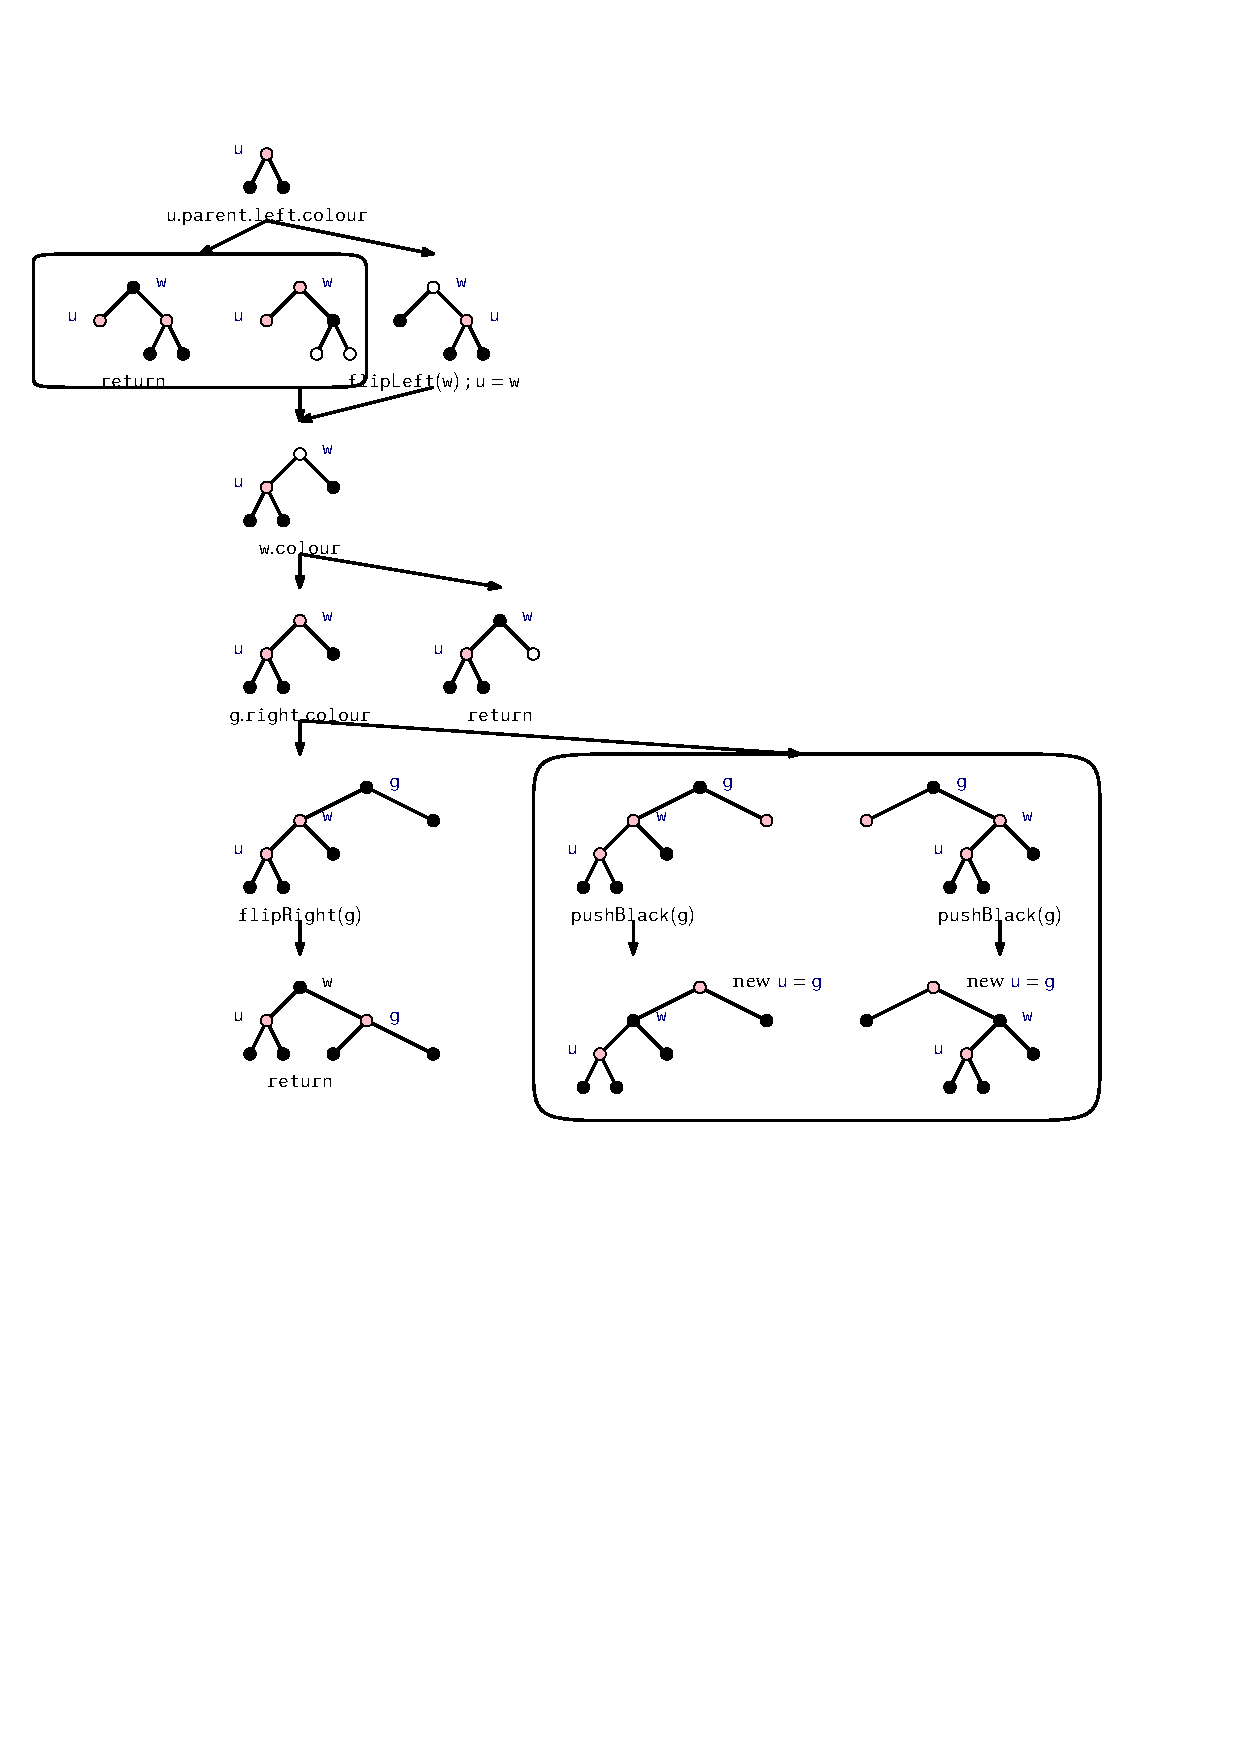
\includegraphics[width=\ScaleIfNeeded]{figs/rb-addfix}
	\end{center}
	\caption{Uma única rodada no processo de fixação da propriedade~2 após
		uma inserção.}
	\figlabel{rb-addfix}
\end{figure}

Se #u# é a raiz da árvore, podemos colorir #u# de preto para restaurar as propriedades. 
Se o irmão de #u# também for vermelho, então o pai de #u# deve ser preto, 
de modo que as propriedades caindo-pra-esquerda e sem-borda-vermelha se mantenham.

Caso contrário, primeiro determinamos se o pai de #u#, #w#, viola a propriedade 
caindo-para-esquerda, e se for o caso, executamos uma operação #flipLeft(w)# e
definimos $#u#=#w#$. Isso nos deixa em um estado bem definido: #u# é o filho
esquerdo de seu pai, #w#, então #w# agora satisfaz a propriedade caindo-pra-esquerda.
Tudo o que resta é garantir a propriedade sem-borda-vermelha em #u#. Nós apenas
temos que nos preocupar em caso de #w# ser vermelho, pois em caso contrário, #u#
já satisfaz a propriedade sem-borda-vermelha.

Uma vez que ainda não terminamos, #u# é vermelho e #w# é vermelho. A propriedade
sem-borda-vermelha (que só é violada por #u# e não por #w#) implica que
o avô de #u#, #g#, existe e é preto. Se o filho direito de #g# for vermelho, então 
a propriedade caindo-para-esquerda garante que ambos os filhos de #g# são vermelhos,
e uma chamada de #pushBlack(g)# faz #g# vermelho e #w# preto. Isso restaura
a propriedade sem-borda-vermelha em #u#, mas pode fazer com que seja violada em #g#,
então todo o processo recomeça com $#u#=#g#$.

Se o filho direito de #g# for preto, então uma chamada para #flipRight(g)# 
faz #w# o pai (preto) de #g# e dá a #w# dois filhos vermelhos, #u# e
#g#. Isso garante que #u# satisfaça a propriedade sem-borda-vermelha e #g#
satisfaça a propriedade caindo-para-esquerda. Neste caso, podemos parar.
\codeimport{ods/RedBlackTree.addFixup(u)}

O método #insertFixup(u)# leva tempo constante por iteração e cada
iteração termina ou move #u# para mais perto da raiz. Assim sendo,
o método #insertFixup(u)# termina após $O(\log #n#)$ iterações em
tempo $O(\log #n#)$.

\subsection{Remoção}

A operação #remove(x)# na #RedBlackTree# é a mais complicada para 
implementar, e isso é verdade para todas as variantes conhecidas de árvore rubro-negra.
Assim como a operação #remove(x)# em uma \texttt{ÁrvoreBináriaDeBusca},
esta operação resume-se a encontrar um nó #w# com apenas um filho,
#u#, e retirar #w# da árvore por fazer #w.parent# adotar #u#.

O problema com isso é que, se #w# for preto, então a propriedade altura-preta
agora será violada em #w.parent#. Podemos evitar esse problema
temporariamente adicionando #w.colour# em #u.colour#. Claro, isso introduz
dois outros problemas: (1)~se ambos #u# e #w# começarem preto, então
$#u.colour#+#w.colour#=2$ (duplo preto), que é uma cor inválida.
Se #w# for vermelho, então ele é substituído por um nó preto #u#, que pode
violar a propriedade caindo-pra-esquerda em $#u.parent#$. Ambos os problemas
podem ser resolvidos com uma chamada do método #removeFixup(u)#.
\codeimport{ods/RedBlackTree.remove(x)}

O método #removeFixup(u)# recebe como entrada um nó #u# cuja cor é preta
(1) ou duplo-preto (2). Se #u# for duplo-preto, então #removeFixup(u)#
executa uma série de rotações e operações de recoloração que movem o
nó duplo preto pra cima da árvore até que possa ser eliminado. Durante este
processo, o nó #u# muda até que, no final deste processo, #u#
aponta para a raiz da subárvore que foi alterada. A raiz desta subárvore
pode ter mudado de cor. Em particular, pode ter ido de vermelho para preto,
então o método #removeFixup(u)# termina ao verificar se o pai de #u# 
viola a propriedade caindo-pra esquerda, e se for o caso, a corrige.
\codeimport{ods/RedBlackTree.removeFixup(u)}

O método #removeFixup(u)# é ilustrado em \figref{rb-removefix}.
Mais uma vez, o seguinte texto será difícil, se não impossível, de se explicar
sem se referir a \figref{rb-removefix}. Cada iteração do loop
em #removeFixup(u)# processa o nó duplo-preto #u# com base em um
de quatro casos:

\begin{figure}
	\begin{center}
		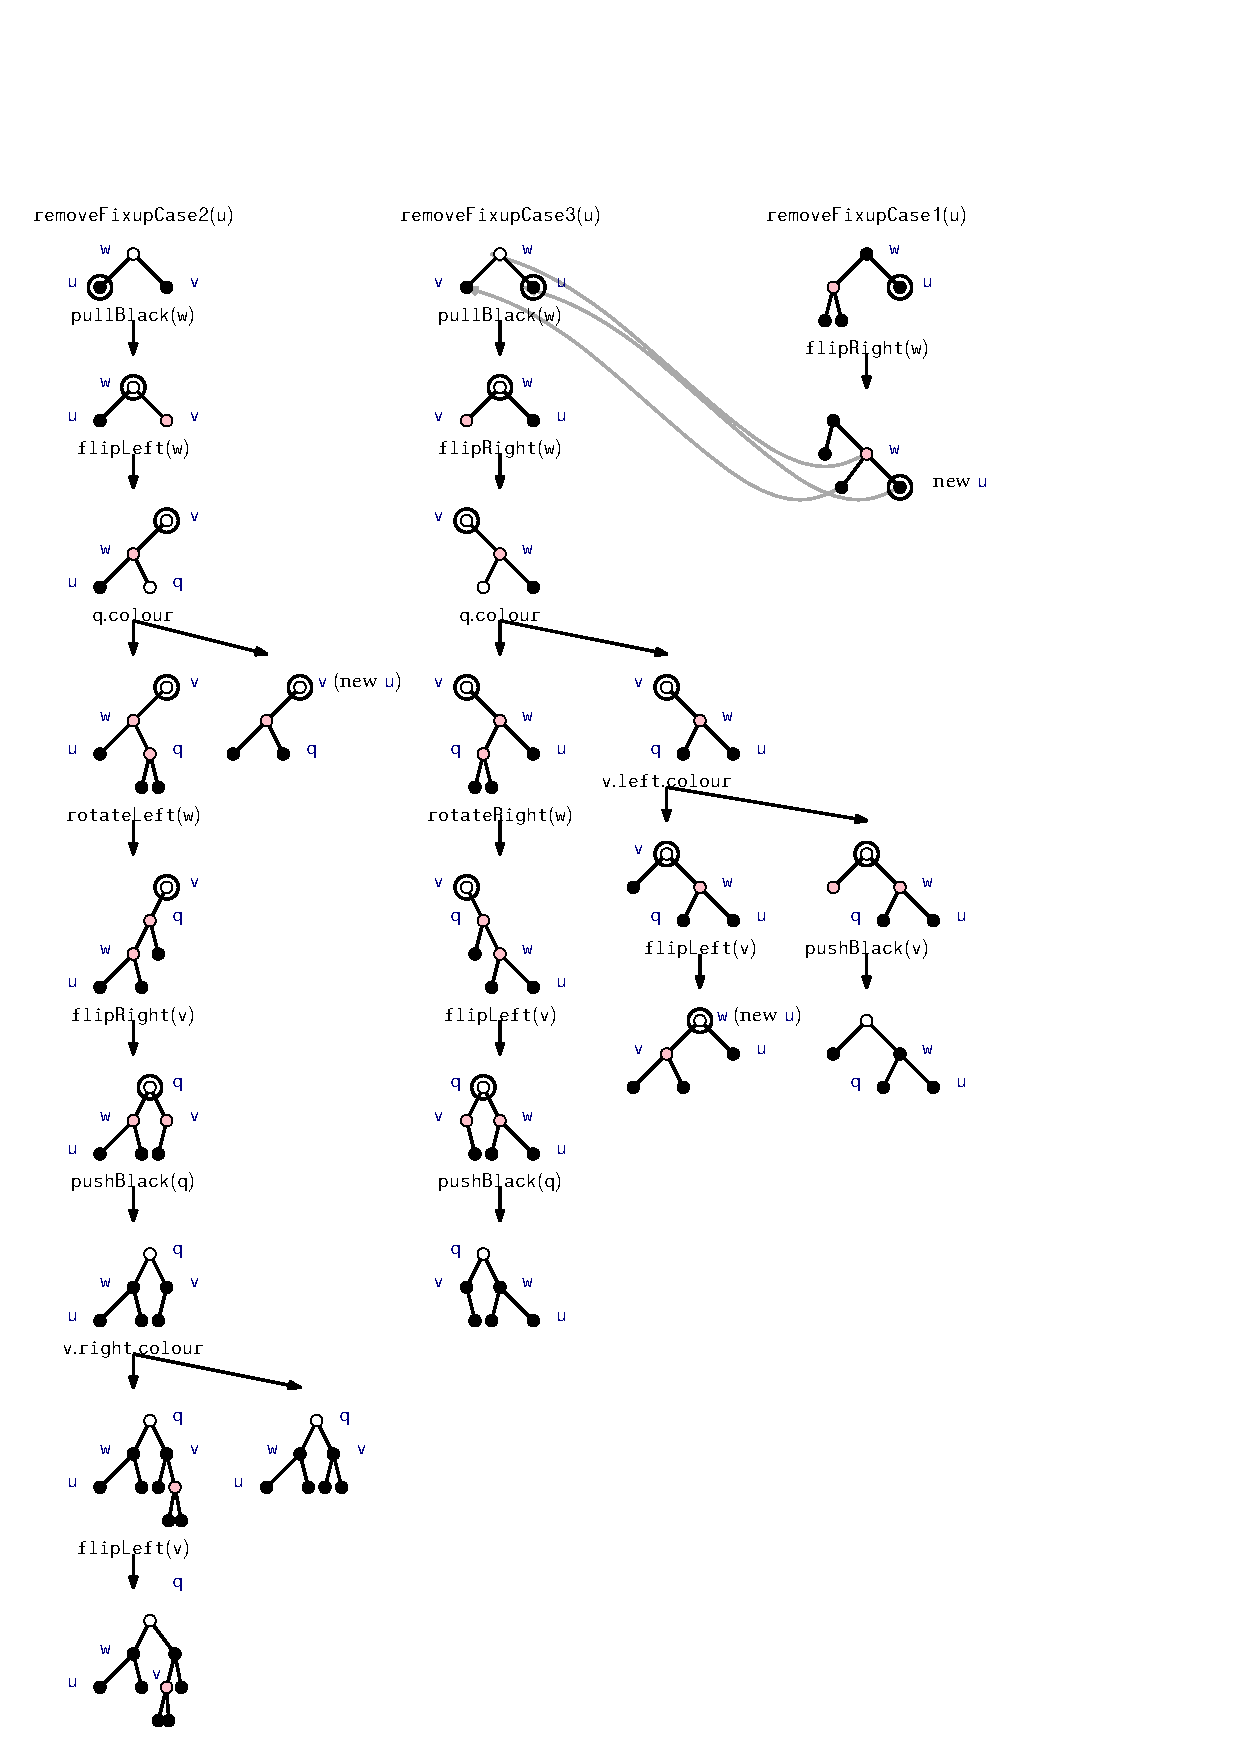
\includegraphics[height=\HeightScaleIfNeeded]{figs/rb-removefix}
	\end{center}
	\caption{Uma única rodada no processo de eliminar um nó duplo-preto
		após uma remoção.}
	\figlabel{rb-removefix}
\end{figure}

\noindent
Caso 0: #u# é a raiz. Este é o caso mais fácil de tratar. Nós recolorimos
#u# para ser preto (isso não viola nenhuma das propriedades das 
árvores rubro-negras).

\noindent 
Caso 1: O irmão de #u#, #v#, é vermelho. Nesse caso, o irmão de #u# é o
filho esquerdo de seu pai, #w# (pela propriedade caindo-pra-esquerda). Nós realizamos
um right-flip direito em #w# e depois prosseguimos para a próxima iteração. Observe que
esta ação faz com que o pai de #w# viole a propriedade caindo-pra-esquerda e
a profundidade de #u# aumente. No entanto, também implica que a próxima
iteração estará no Caso~3 com #w# colorido de vermelho. Ao examinar o
Caso~3 abaixo, veremos que o processo irá parar durante a próxima iteração.
\codeimport{ods/RedBlackTree.removeFixupCase1(u)}

\noindent 
Caso 2: O irmão de #u#, #v#, é preto, e #u# é o filho esquerdo de seu
pai, #w#. Nesse caso, chamamos #pullBlack(w)#, fazendo #u# preto,
#v# vermelho e escurecendo a cor de #w# para preto ou duplo-preto.
Neste ponto, #w# não satisfaz a propriedade caindo-pra-esquerda, então 
nós chamamos #flipLeft(w)# para corrigir isso.

Neste ponto, #w# é vermelho e #v# é a raiz da subárvore com a qual nós 
começamos. Precisamos verificar se #w# faz com que a propriedade sem-borda-vermelha 
seja violada. Fazemos isso inspecionando o filho direito de #w#, #q#. Se #q#
é preto, então #w# satisfaz a propriedade sem-borda-vermelha e podemos continuar
a próxima iteração com $#u#=#v#$.

Caso contrário (#q# é vermelho), tanto a propriedade sem-borda-vermelha quanto 
a caindo-pra-esquerda são violadas em #q# e #w#, respectivamente.
A propriedade caindo-pra-esquerda é restaurada com uma chamada de
#rotateLeft(w)#, mas a propriedade sem-borda-vermelha
ainda é violada. Neste ponto, #q# é o filho esquerdo de
#v#, #w# é o filho esquerdo de #q#, #q# e #w# são vermelhos e #v#
é preto ou duplo-preto. A #flipRight(v)# faz #q# o pai de
ambos #v# e #w#. Seguindo com um #pushBlack(q)#, colore #v#
e #w# de preto e define a cor de #q# de volta para a cor original de #w#.

Neste ponto, o nó duplo-preto foi eliminado e as propriedade sem-borda-vermelha
e altura-preta estão restabelecidas. Apenas um problema possível: o filho direito de #v# pode ser vermelho, 
caso no qual a propriedade caindo-pra-esquerda seria violada. Verificamos isso e
executamos um #flipLeft(v)# para corrigi-la, se necessário.
\codeimport{ods/RedBlackTree.removeFixupCase2(u)}

\noindent
Caso 3: o irmão de #u# é preto e #u# é o filho certo de seu pai, #w#. 
Este caso é simétrico ao Caso~2 e é tratado principalmente da mesma maneira.
As únicas diferenças vêm do fato de que a propriedade caindo-pra-esquerda
é assimétrica, por isso requer uma manipulação diferente.

Como antes, começamos com uma chamada de #pullBlack(w)#, o que torna #v# vermelho
e #u# black. Uma chamada de #flipRight(w)# promove #v# para a raiz da
subárvore. Neste ponto #w# é vermelho, e o código se ramifica de duas maneiras
dependendo da cor do filho esquerdo de #w#, #q#.

Se #q# estiver vermelho, o código termina exatamente da mesma maneira que
o Caso~2 termina, mas é ainda mais simples já que não há perigo de #v# não
satifazer a propriedade caindo-pra-esquerda.

O caso mais complicado ocorre quando #q# é preto. Nesse caso,
nós examinamos a cor do filho esquerdo de #v#. Se for vermelho, então #v# tem
dois filhos vermelhos e seu preto extra podem ser postos pra baixo com uma chamada
de #pushBlack(v)#. Neste ponto, #v# agora tem a cor original de #w#, e assim
terminamos.

Se o filho esquerdo de #v# for preto, então #v# viola a propriedade caindo-pra-esquerda,
e restauramos isso com uma chamada de #flipLeft(v)#. Depois, devolvemos o
nó #v# para que a próxima iteração de #removeFixup(u)# continue
com $#u#=#v#$.
\codeimport{ods/RedBlackTree.removeFixupCase3(u)}.

Cada iteração de #removeFixup(u)# leva tempo constante. Os casos~2 e 3
terminam ou movem #u# para mais perto da raiz da árvore. O Caso~0 (onde
#u# é a raiz) sempre termina, o e Caso~1 leva imediatamente para Caso~3,
que também termina. Como a altura da árvore é de no máximo $2\log#n#$,
concluímos que existem no máximo $O(\log #n#)$ iterações de #removeFixup(u)#,
então #removeFixup(u)# é executado em tempo $O(\log #n#)$.


\section{Resumo}
\seclabel{redblack-summary}

O seguinte teorema resume o desempenho da estrutura de dados #RedBlackTree#:

\begin{thm}
	Uma #RedBlackTree# implementa a interface #SSet# e
	suporta as operações #add(x)#, #remove(x)# e #find(x)# em tempo
	de pior caso $O(\log#n#)$ por operação.
\end{thm}

Não incluído no teorema acima é o seguinte bônus extra:

\begin{thm}\thmlabel{redblack-amortized}
	Começando com uma #RedBlackTree# vazia, qualquer seqüência de $ m$
	operações #add(x)# e #remove(x)# resultam em um tempo total gasto de $O(m)$
	durante todas as chamadas de #addFixup(u)# e #removeFixup(u)#.
\end{thm}

Nós apenas esboçamos uma prova de \thmref{redblack-amortized}. Comparando
#addFixup(u)# e #removeFixup(u)# com os algoritmos para adicionar ou
remover uma folha em uma árvore 2-4, podemos nos convencer de que essa
propriedade é herdada de uma árvore 2-4. Em particular, se pudermos mostrar
que o tempo total gasto dividindo, mesclando e pegando emprestado em uma
ávore 2-4 é $O(m)$, então isso implica \thmref{redblack-amortized}.

A prova deste teorema para árvores 2-4 usa o método
potencial
\index{potential method}%
de análise amortizada.\footnote{Veja a prova de
	\lemref{dualarraydeque-amortized} e \lemref{selist-amortized} para
	outras aplicações do método potencial.} Defina o potencial de um
nó interno #u# em uma árvore 2-4 como
\[
\Phi(#u#) = 
\begin{cases} 
1 & \text{se #u# tem 2 filhos} \\ 
0 & \text{se #u# tem 3 filhos} \\ 
3 & \text{se #u# tem 4 filhos}  
\end{cases}
\]
e o potencial de uma árvore 2-4 como a soma dos potenciais dos seus nós.
Quando ocorre uma divisão, é porque um nó com quatro filhos se torna
dois nós, com dois e três filhos. Isso significa que o potencial total 
cai em $3-1-0 = 2$. Quando ocorre uma mesclagem, dois nós que tinham 
dois filhos são substituídos por um nó com três filhos.
O resultado é uma queda de $2-0=2$ no potencial. Portanto, para 
cada divisão ou mesclagem, o potencial diminui em dois.

Agora perceba que, se ignorarmos a divisão e a mesclagem de nós, existe
apenas um número constante de nós cujo número de filhos é alterado 
pela adição ou remoção de uma folha. Ao adicionar um nó, um nó tem
o número de filhos aumentado em um, aumentando o potencial por
no máximo três. Durante a remoção de uma folha, um nó tem seu número
de filhos diminuido em um, aumentando o potencial por até um,
e dois nós podem estar envolvidos em uma operação de pegar emprestado,
aumentando seu potencial total por até um.

Para resumir, cada mesclagem e divisão causam o potencial de cair por
ao menos dois. Ignorando a mesclagem e a divisão, cada adição ou remoção
faz com que o potencial aumente por até três, e o potencial é sempre
não negativo. Portanto, o número de divisões e fusões causadas por $m$
adições ou remoções em uma árvore inicialmente vazia é no máximo $3m/2$.
\thmref{redblack-amortized} é uma conseqüência dessa análise e a
correspondência entre árvores 2-4 e árvores rubro-negras.

\section{Discussão e Exercícios}

Árvores rubro-negras foram introduzidas pela primeira vez por Guibas e Sedgewick \cite{gs78}.
Apesar da sua alta complexidade de implementação, elas são encontradas em algumas
das bibliotecas e aplicações mais utilizadas. A maioria das apostilas de algoritmos e
e estruturas de dados discutem algumas variantes de árvores rubro-negras.

Andersson \cite{a93} descreve uma versão de árvores balanceadas
que  são semelhantes às árvores rubro-negras, mas tem a restrição adicional
de qualquer nó ter  no máximo um filho vermelho. Isso implica que essas árvores
simulam árvores 2-3 ao invés de árvores 2-4. Elas são significativamente mais simples,
no entanto, que a estrutura #RedBlackTree# apresentada neste capítulo.

Sedgewick \cite{s08} descreve duas versões de árvores rubro-negras caindo pra esquerda. 
Estas usam a recursão junto com uma simulação de divisão de cima para baixo
e mesclando em árvores 2-4. A combinação dessas duas técnicas fazem
um código curto e elegante.

Uma estrutura de dados relacionada e mais antiga é a \emph{ávore AVL} \cite{avl62}.
\index{AVL tree}%
As árvores de AVL são \emph{height-balanced}:
\index{height-balanced}%
\index{binary search tree!height balanced}%
Em cada nó $u$, as alturas
da subárvore enraizada em #u.left# e da subárvore enraizada em #u.right#
diferem por mais de um. Segue-se imediatamente que, se $F(h)$ for o
número mínimo de folhas em uma árvore de altura $h$, então $F(h)$ obedece a
recorrência de Fibonacci
\[
F(h) = F(h-1) + F(h-2)
\]
com casos base $F(0)=1$ and $F(1)=1$. Isso significa que $F(h)$ é aproximadamente
$\varphi^h/\sqrt{5}$, onde $\varphi=(1+\sqrt{5})/2\approx1.61803399$ é o
\emph{coeficiente de ouro}. (Mais precisamente, $|\varphi^h/\sqrt{5} - F(h)|\le 1/2$.)
Argumentando como na prova de \lemref{twofour-height}, isso implica
\[
h \le \log_\varphi #n# \approx 1.440420088\log #n# \enspace ,
\]
então as árvores AVL têm altura menor do que árvores rubro-negras. O balanceamento de 
altura pode ser mantido durante as operações #add(x)# e #remove(x)#
ao caminhar de volta ao caminho da raiz e realizar uma operação
de rebalanceamento em cada nó #u# onde a altura das subarvores esquerda e direita de #u#
diferem em dois. Veja \figref{avl-rebalance}.

\begin{figure}
	\begin{center}
		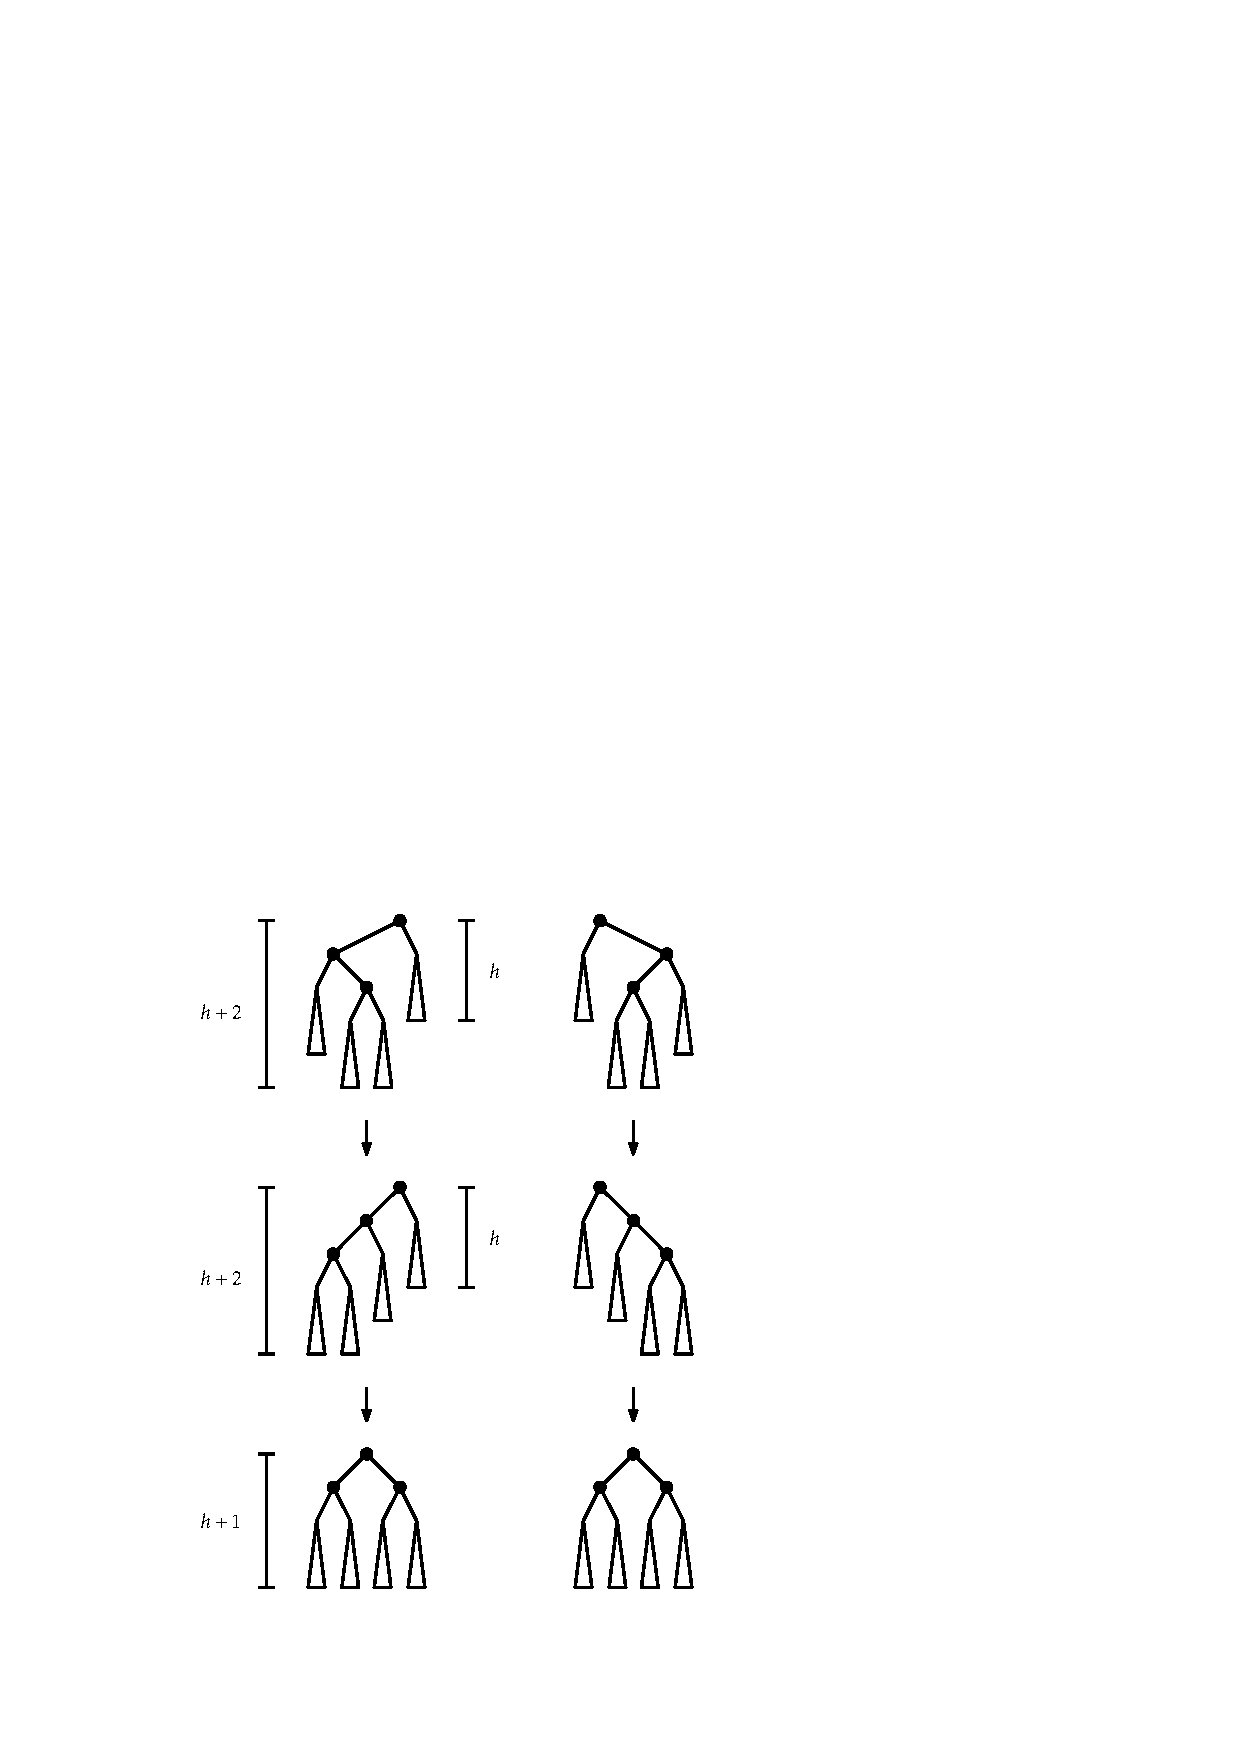
\includegraphics[scale=0.90909]{figs/avl-rebalance}
	\end{center}
	\caption{Reequilibrando em uma árvore AVL. No máximo, duas rotações são necessárias
		para converter um nó cujas subárvores tenham uma altura de $h$ and $h+2$ em um nó
		cujas subárvores têm uma altura de no máximo $h+1$.}
	\figlabel{avl-rebalance}
\end{figure}

As variantes de Andersson e de Sedgewick da árvore rubro-negra e as árvores AVL 
são mais simples de implementar do que a estrutura #c# 
definida aqui. Infelizmente, nenhuma delas pode garantir que o tempo amortizado 
gasto rebalanceamento é $O(1)$ por atualização. Em particular, não há analogias
de \thmref{redblack-amortized} para essas estruturas.

\begin{figure}
	\centering{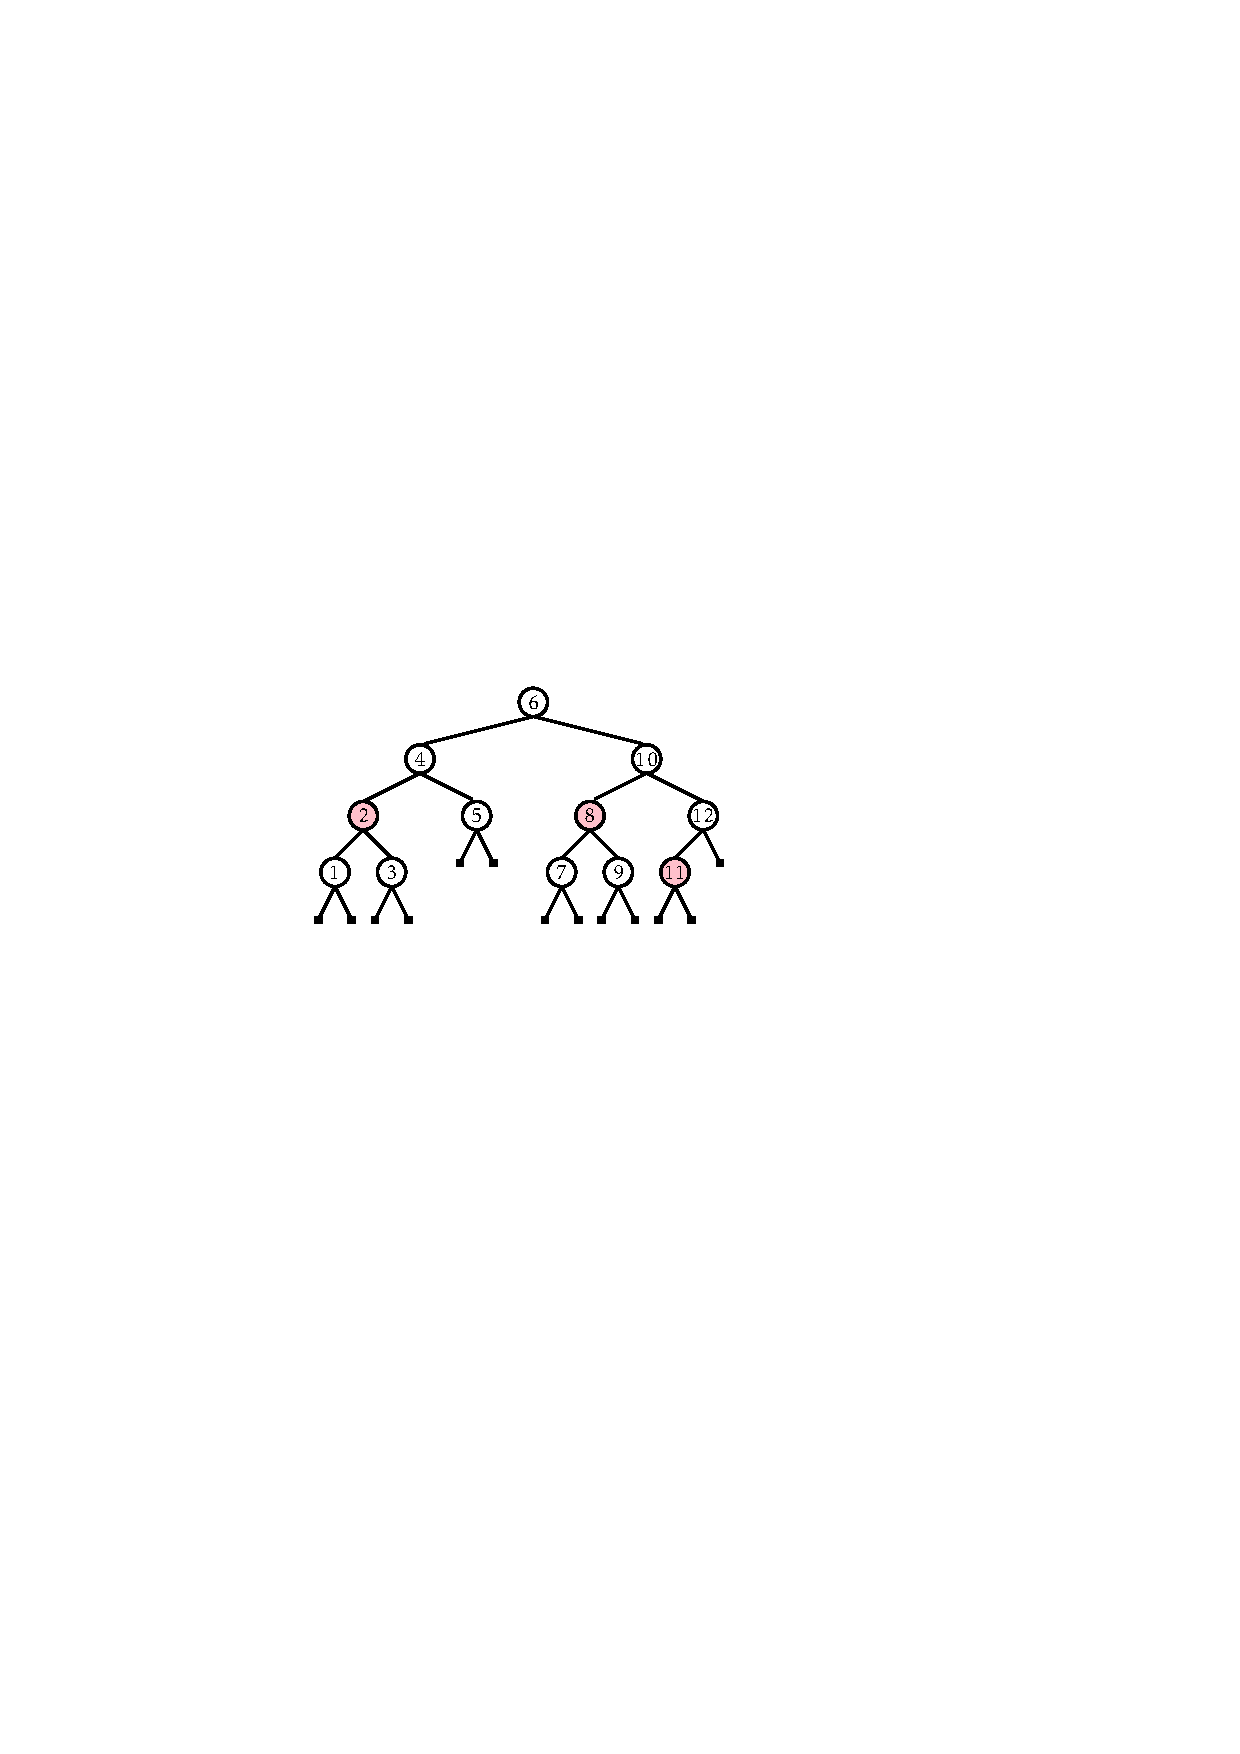
\includegraphics[scale=0.90909]{figs/redblack-example}}
	\caption{Uma árvore rubro-negra para praticar.}
	\figlabel{redblack-example2}
\end{figure}

\begin{exc}
	Ilustre a árvore 2-4 que corresponde à #RedBlackTree# em
	\figref{redblack-example2}.
\end{exc}

\begin{exc}
	Ilustre a adição de 13, depois de 3.5, e depois de 3.3 na #RedBlackTree#
	em \figref{redblack-example2}.
\end{exc}

\begin{exc}
	Ilustre a remoção de 11, depois de 9, e depois de 5 na #RedBlackTree# em
	\figref{redblack-example2}.
\end{exc}

\begin{exc}
	Mostre que, para valores arbitrariamente grandes de #n#, há vermelho-preto
	árvores com #n# nós com altura de $2\log #n#-O(1)$.
\end{exc}

\begin{exc}
	Considere as operações #pushBlack(u)# e #pullBlack(u)#. O que fazem 
	essas operações para a árvore 2-4 subjacente que está sendo simulada
	pela árvore rubro-negra?
\end{exc}

\begin{exc}
	Mostre que, para valores arbitrariamente grandes de #n#, existem sequências
	de operações #add(x)# e #remove(x)# que ocasionam árvores vermelho-pretas
	com #n# nós de altura $2\log #n#-O(1)$.
\end{exc}



\begin{exc}
	Por que o método #remove(x)# na implementação #RedBlackTree#
	executa a atribuição #u.parent=w.parent#? Isso já não deveria  
	estar feito pela chamada de #splice(w)#?
\end{exc}

\begin{exc}
	Suponha que uma árvore 2-4, $T$, tenha $#n#_\ell$ folhas e $#n#_i$ nós internos.
	\begin{enumerate}
		\item Qual é o valor mínimo de $#n#_i$ em função de $#n#_\ell$?
		\item Qual é o valor máximo de $#n#_i$ em função de $#n#_\ell$?
		\item Se $T'$ é uma árvore rubro-negra que representa $T$, então, quantos nós
		vermelhos tem $T'$?
	\end{enumerate}
\end{exc}

\begin{exc}
	Suponha que você tenha uma árvore binária de busca com #n# nós e 
	altura de no máximo $2\log #n#-2$. É sempre possível colorir os nós 
	vermelhos e pretos de modo que a árvore satisfaça as propriedades altura-preta 
	e sem-borda-vermelha? Se positivo, também pode ser feito para satisfazer a
	a propriedade caindo-pra-esquerda?
\end{exc}

\begin{exc} \exclabel{redblack-merge}
	Suponha que você tenha duas árvores vermelho-pretas $T_1$ and $T_2$ de
	mesma altura preta, $h$, e tal que a maior chave em $T_1$ é menor
	do que a menor chave em $T_2$. Mostre como combinar $T_1$ e $T_2$
	em uma única árvore rubro-negra em tempo $O(h)$.
\end{exc}

\begin{exc}
	Estenda sua solução para \excref{redblack-merge} para o caso em que as
	duas árvores $T_1$ and $T_2$ têm alturas pretas diferentes, $h_1\neq h_2$.
	O tempo de execução deve ser $O(\max\{h_1,h_2\})$.
\end{exc}



\begin{exc}
	Prove que, durante uma operação #add(x)#, uma árvore AVL deve executar
	no máximo, uma operação de rebalanceamento (que envolve no máximo duas rotações;
	veja \figref{avl-rebalance}). Dê um exemplo de uma árvore AVL e uma
	operação #remove(x)# naquela árvore que requer operações de rebalanceamento
	da ordem de $\log#n#$
\end{exc}

\begin{exc}
	Implemente uma classe #AVLTree# que implementa árvores AVL conforme descrito
	acima. Compare seu desempenho com o da implementação #RedBlackTree#. 
	Qual implementação tem uma operação #find(x)# mais rápida?
\end{exc}

\begin{exc}
	Projete e implemente uma série de experimentos que comparam a performance relativa
	de #find(x)#, #add (x)# e #remove (x)# para as implementações #SSet# de #SkiplistSSet#,
	#ScapegoatTree#, #Treap# e #RedBlackTree#. Certifique-se de incluir
	vários cenários de teste, incluindo casos em que os dados são aleatórios,
	já ordenado, são removidos em ordem aleatória, são removidos em ordem ordenada,
	e assim por diante.
\end{exc}
